\documentclass[10pt, a4paper]{article}
\usepackage{subfigure,layout, amssymb, graphicx, textcomp, url, color}
\newcommand{\comment}[1]{} % en kommentar.
\newcommand{\partners}{\emph{Partners:~}}
\newcommand{\period}{\emph{Period:~}}
\newcommand{\aabstract}[1]{\emph{Abstract:~}#1}
\newcommand{\aauthor}[1]{\emph{Author:~}#1\\}
\newcommand{\aauthors}[1]{\emph{Authors:~}#1\\}
\newcommand{\bbook}[1]{\emph{Book:}~#1\\}
\newcommand{\ccomment}[1]{\emph{Comment:~}#1\\}
\newcommand{\cconference}[1]{\emph{Conference:~}#1}
\newcommand{\eeditor}[1]{\emph{Editor:~}#1\\}
\newcommand{\eeditors}[1]{\emph{Editors:~}#1\\}
\newcommand{\ffunding}[1]{\emph{Funding:~}#1\\}
\newcommand{\jjournal}[1]{\emph{Journal:~}#1\\}
\newcommand{\ppartner}[1]{\emph{Partner:~}#1\\}
\newcommand{\ppartners}[1]{\emph{Partners:~}#1\\}
\newcommand{\ppublisher}[1]{\emph{Publisher:~}#1}
\newcommand{\pperiod}[1]{\emph{Period:~}#1\\}
\newcommand{\ttitle}[1]{\item \textbf{#1}\\}
\newcommand{\cba}{CBA}
\newcommand{\uu}{UU}

\begin{document}

\newcommand{\commentfigure}[1]{}
\newcommand{\researcharea}[1]{\subsection{#1}}

\section{Research}\label{research}
\label{research_proj}
{\large
Our research activities are conducted in a large number of projects, both very application oriented and very theoretical, both large and small, both long-running and short-lived. Our largest application field is, since a long time, biomedicine, both analysis of microscopic images of everything from proteins to tissue samples and analysis of whole organs or the whole body. There are also other applications, especially the analysis of old, handwritten documents and forest industry applications. As this is the last year SLU will be involved in CBA, the latter will naturally end in their present form, but some may continue in new constellations. The tools we use are general image analysis tools, graphical tools for visualisation and haptic tools. In addition to developing or inventing the tools we need for our applications, we also do theoretical research in discrete geometry and mathematical morphology, both in two and three dimensions. 

In Section \ref{partners} we have collected all our research partners, international and national, with whom we had active co-operation in the form of either a joint project or a joint publication, during the year. 

%Our research activities are conducted in a large number of projects, both very application oriented and theoretical, both large and small, both long-running and short. More specifically, we worked on 47 projects this year, out of which 40 were continuing projects, there were 7 new projects and 14 projects were completed before 2014. Our largest application field is biomedicine, with many projects developing methods for analysing microscopic images of molecules, viruses, cells, and tissue. In addition we also have much going on in analysis and visualization of 3D medical images. In the latter case we develop haptic tools for interactive exploration of such images. We are also active in the analysis of wood and wood fibre based materials. In addition to these areas especially mentioned in our charter we are involved in other applications, the biggest of which is analysis of old, handwritten texts. There are also projects for the urban and rural environments -- and for tracking bees. In our application projects we have a partner with a set of images and a problem getting information from them, a problem interesting enough to generate new analysis methods. We also develop new, general theory for image analysis and visualization, especially in digital geometry and mathematical morphology and usually in volume images, but not as much as we would like to. The reason is that it is much easier to get grants for applications of image analysis than for image analysis itself. 

%In Section \ref{partners} we have collected all partners, national and international, with which we had active co-operation in 2013. They can all also be found somewhere else in this report.}
\vfill

\subsection{Analysis of microscopic biomedical images}
\begin{enumerate}
	\setcounter{enumi}{0}
% AAA

\item
\label{proj:PVS2}
\textbf{Identification of Highly Pathogenic Viruses in Transmission Electron Microscopy Images}\\
Gustaf Kylberg, Ida-Maria Sintorn, Ewert Bengtsson, Gunilla Borgefors\\
\ppartners{Vironova AB; Delong Instruments, Brno, Czech Republic; Ali Mirazimi, Kjell-Olof H\"{o}glund, Centre for Microbiological Preparedness; Swedish Institute for Infectious Disease Control (SMI)}
\ffunding{2008--2011 Swedish Civil Contingencies Agency (MSB), Swedish Defense Materiel Administration (FMV), Swedish Agency for Innovative Systems (VINNOVA). 2011--2013 Eurostar project}
\pperiod{0801--}
\aabstract{This project aims at automating the virus identification process in high resolution TEM images. This, in combination with Project \ref{proj:PVS1} to create a rapid, objective, and user independent virus diagnostic system. The identification task consists of method development for segmenting virus particles with different shapes and sizes and extracting descriptive features of both shape and texture to enable the classification into virus species. Texture features such as variants of Local Binary Patterns and Regional Moments (filter banks constructed from orthogonal moments), are being evaluated on virus textures as well as other texture datasets to get a deeper understanding of the discriminant power of the features under different conditions. A paper comparing, combining and evaluating the discriminating power of local texture descriptors for virus classification was presented at the International Conference on Pattern Recognition (ICPR) in Stockholm in August and Gustaf Kylberg defended his PhD thesis closely linked to this project in March 2014.} 

% BBB

\item
\label{proj:PVS1}
\textbf{The MiniTEM Project - Development of a Desk-top TEM with Automated Image Acquisition}\\ 
Gustaf Kylberg, Ida-Maria Sintorn, Ewert Bengtsson, Gunilla Borgefors\\
\ppartners{Vironova AB; Delong Instruments, Brno, Czech Republic}
\ffunding{Eurostar project}
\pperiod{1107--}
\aabstract{Transmission electron microscopy (TEM) is an important clinical diagnostic and material analysis tool. Transmission electron microscopes are expensive, complex, sensitive and bulky machines, often housed in specially built rooms to avoid vibrations affecting the imaging process. They are to a very large extent manually operated, meaning that an expert in electron microscopy and preferably also in the  application at hand needs to perform the analysis at the microscope, an often very time consuming task. 
	
This project aimed at developing the MiniTEM, a desk-top low voltage TEM designed for imaging biological samples, with a high degree of automation regarding instrument alignment, image acquisition and analysis. The goal was a small, cheap, robust, and easy to use system that requires no more training than any simple lab equipment, and can be hosted in any office or lab (even mobile).
	
Automating the image acquisition process is key for reducing the manual input and making the imaging and analysis more objective. Within the project different strategies for automating the image acquisition were developed and investigated. The first was acquisition of images at random positions on the grid. The second was to search for a specific structure/object and only acquire (store) the images containing the structure/object of interest. The third was similar to the second approach but embedded in a multi-scale approach with the goal to make the acquisition more efficient.
	
The MiniTEM was launched and displayed at the International Microscopy Congress in Prague in September. One instrument was at the conference site and a second piece, physically in Stockholm, was operated remotely from Prague. Abstracts and posters about the project, the developled image analysis methods, and actual instrument, have been presented at various international and national conferences and meetings throughout the year. Gustaf Kylberg successfully defended his PhD thesis early 2014, which was closely linked to this project. The MiniTEM, its GUI and two example images showing a mixture of typical clinical application areas are shown in Figure \ref{fig:miniTEM}.}

\begin{figure}[!h]
	\centering
	
	\subfigure[]{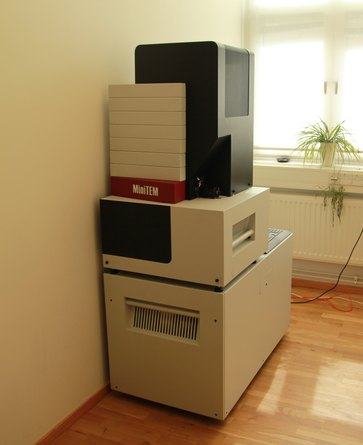
\includegraphics[width=0.4\linewidth]{figures/research/MiniTEM_Instrumentsmallercut.png}}
	\subfigure[]{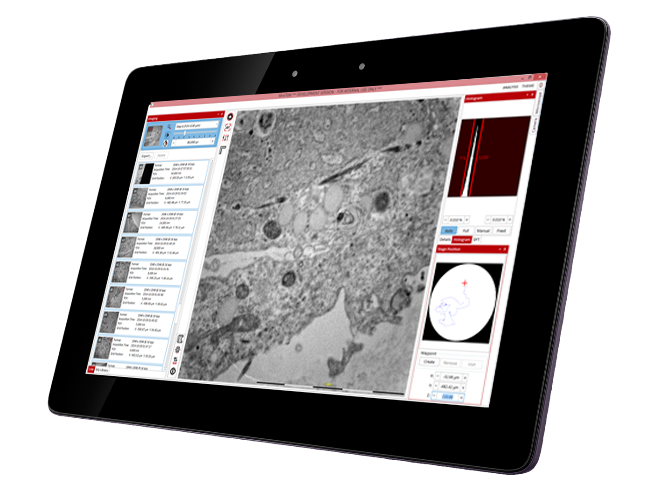
\includegraphics[width=0.4\linewidth]{figures/research/MiniTEMGUIAR2013screenshot.png}}\\
	\subfigure[]{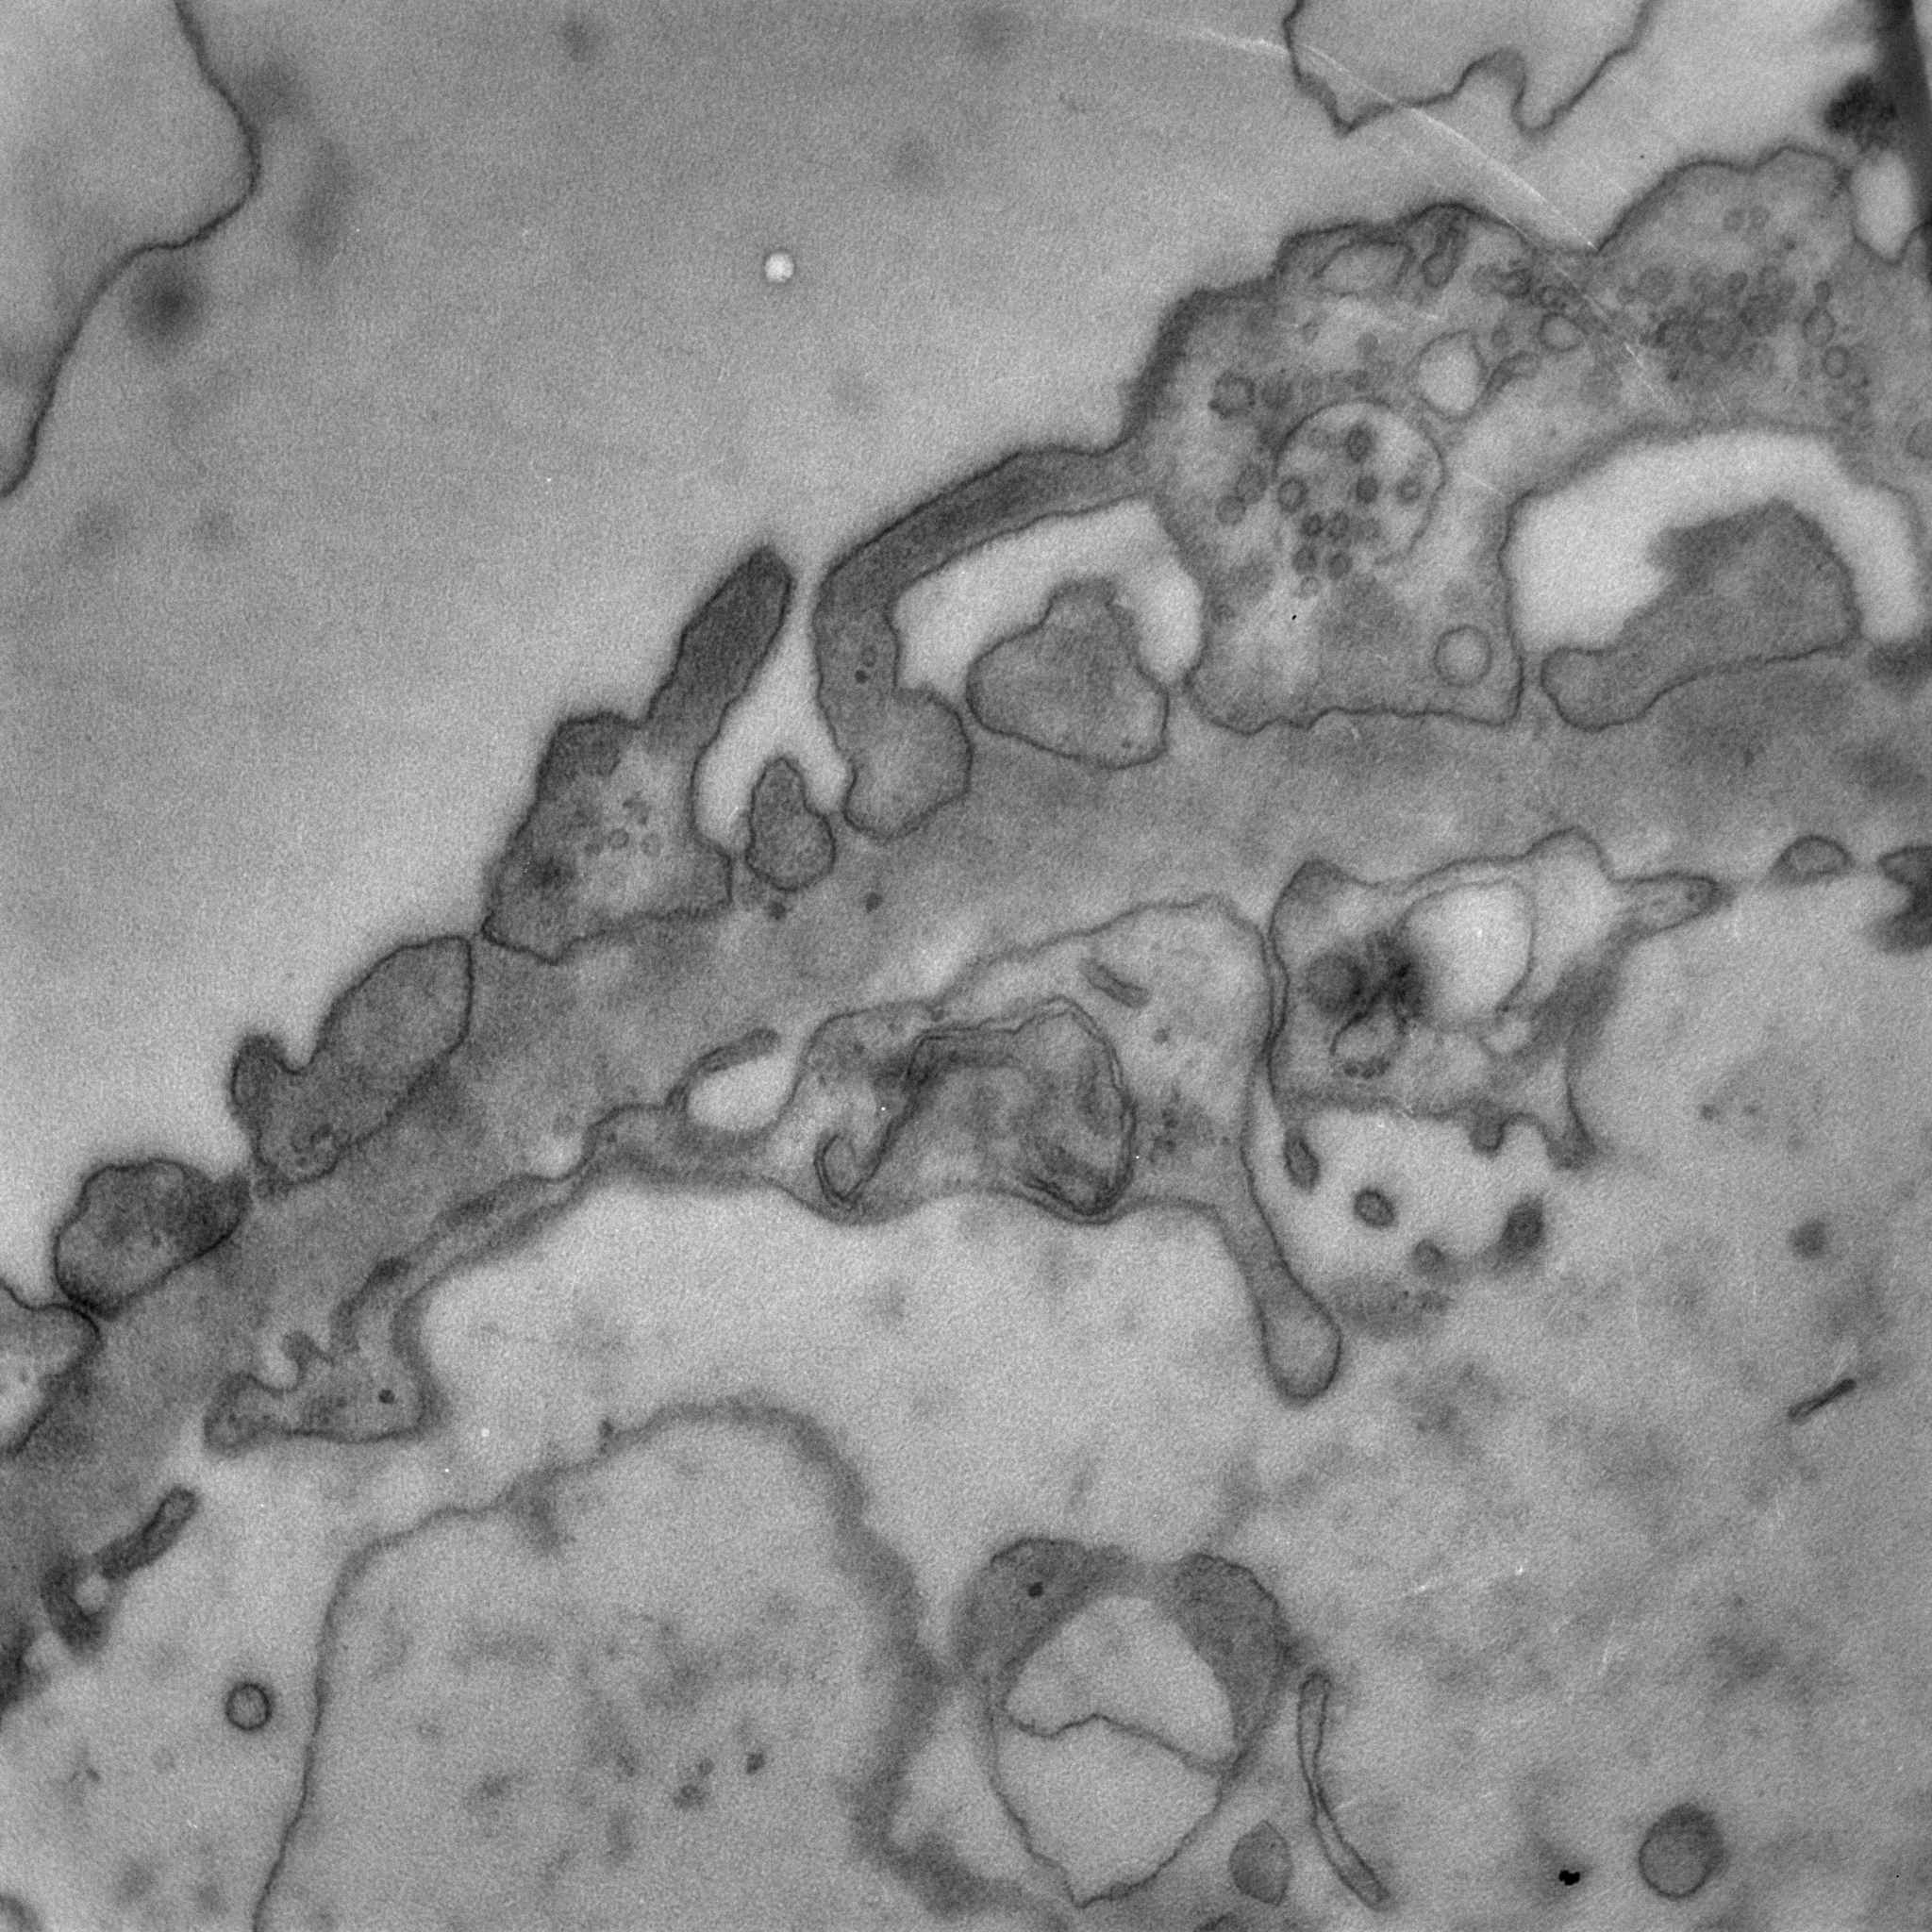
\includegraphics[width=0.4\linewidth]{figures/research/MiniTEMKidneyforAR2013.png}}
	\subfigure[]{\includegraphics[width=0.4\linewidth]{figures/research/MiniTEMAdenoRotaAr2013_FOV500nm.png}}
		\caption{The MiniTEM instruments, its GUI and images of a filtering membrane in a kidney section and a mixture of Adeno and Rota viruses. \label{fig:miniTEM}}
	
	\end{figure}

%\begin{figure*}[!h]
%\centering
%\subfigure[]{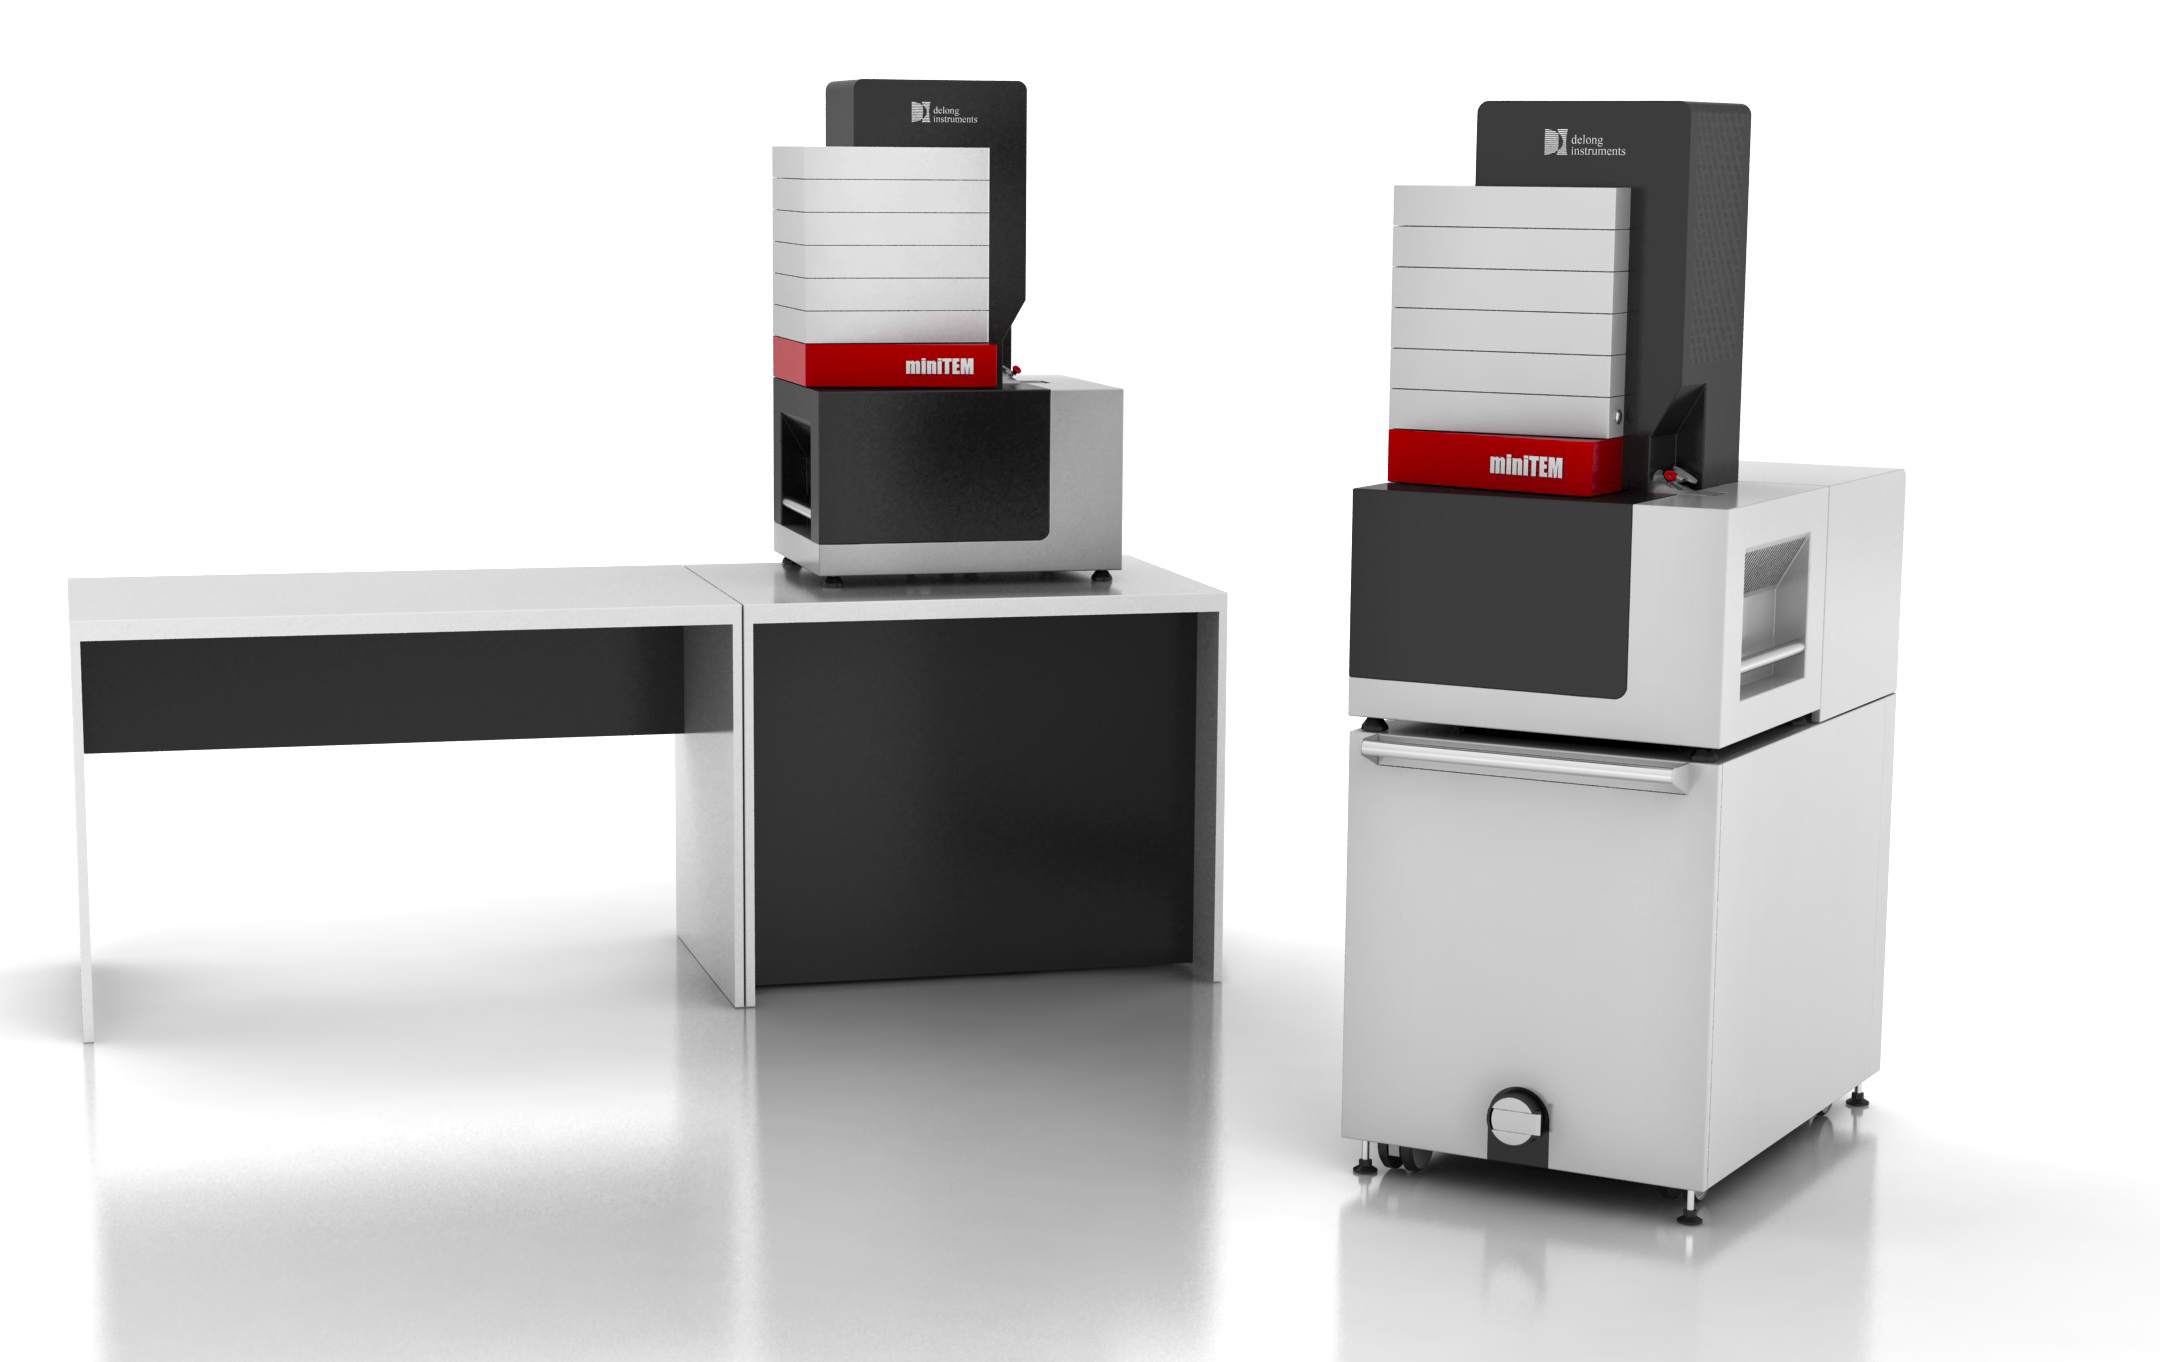
\includegraphics[width=0.36\linewidth]{figures/research/miniTEMLarge.png}}
%\subfigure[]{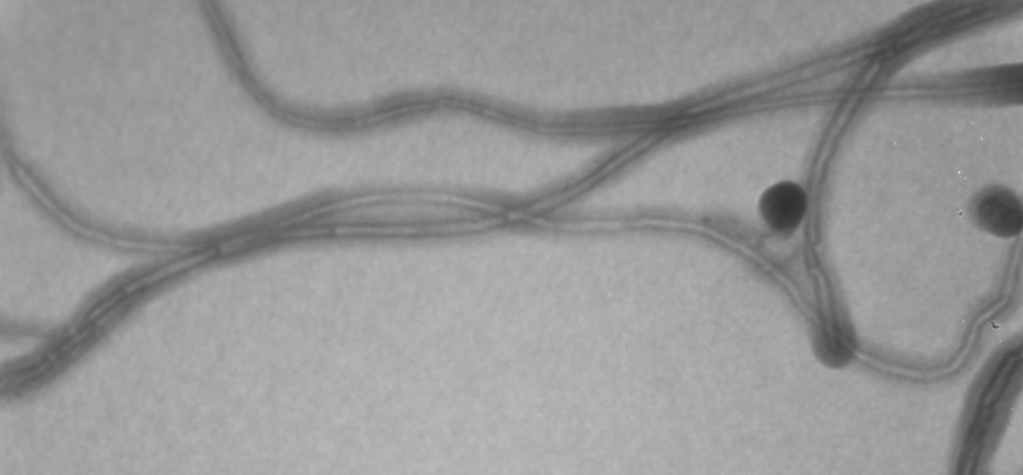
\includegraphics[width=0.48\linewidth]{figures/research/miniTEMnanotubulescutwider.png}}
%\caption{Desk-top and mobile version of the miniTEM (left). Nanotubes, approximately 15nm thick, the first image acquired with the miniTEM (right).}
%\label{fig:miniTEM}
%\end{figure*}

% CCC

\item 
\textbf{Detection and Localization of Florescent Signals in STORM Data Using Compressed Sensing}\\
Omer Ishaq, Alexandra Pacureanu, Carolina W\"{a}hlby\\
\ppartners{Johan Elf, Gustaf Ullman, Fredrik Persson, Dept.~of Cell \& Molecular Biology, UU}
\ffunding{SciLifeLab Uppsala, eSSENCE, VR junior researcher grant to CW}
\pperiod{1211--}
\aabstract{Stochastic optical reconstruction microscopy (STORM) is a super-resolution microscopy image acquisition technique for single-molecule localization. Like other stochastic super-resolution microscopy techniques it incorporates a trade-off between spatial- and temporal-resolution. Recently, a compressed-sensing (CS) based variant of STORM, called FasterSTORM, has been developed which substantially increases the temporal sampling of a stack of STORM image frames. This improvement is realized by increasing the density of activated fluorophores in each frame, followed by a subsequent CS-based retrieval of single-molecule positions even with overlapping fluorescent signals. However, the CS-based retrieval/decoding step is time consuming and can take as much as three hours for each image frame. We have accelerated the FasterSTORM method through parallel processing on multi-core processors. Additionally, we have tested and tried a number of L1-solvers for CS-based recovery of molecule positions. We are in the process of comparing the performance of the FasterSTORM against a wavelet-based approach to localize fluorescent signals in time-lapse images of bacterial cells.
	
In 2014, a paper comparing convex and greedy solvers and evaluating the sensitivity of the FasterSTORM to estimation bias of the point spread function (PSF) was accepted for oral presentation at the $22^{nd}$ International Conference on Pattern Recognition (ICPR 2014).}

%DDD

\item 
\textbf{\emph{In Situ} Sequencing of mRNA}\\
Carolina W\"{a}hlby, Alexandra Pacureanu, Petter Ranefall \\
\ppartners{Mats Nilsson, Rongqin Ke, Marco Mignardi, Thomas Hauling, Xiaoyan Qian, SciLifeLab Stockholm/Stockholm University}
\ffunding{SciLifeLab Uppsala; TN-faculty, UU}
\pperiod{1109--}
\aabstract{Profiling of gene expression is prerequisite for understanding the function of cells, organs and organisms, in health and disease. The sequencing techniques currently in use rely on homogenization of the samples. Therefore, the obtained information represents either the average expression profile of the tissue sample or expression profiles of isolated single cells. Our collaborators have developed a new molecular method, enabling \emph{in situ} sequencing of mRNA, so that protein expression can be observed directly in cultured cells or tissue samples. We have developed image analysis tools for automated analysis of sequencing data, mapping, and visualization of gene expression patterns (Figure \ref{fig:carolina_insitu}). In 2013 we presented the work as part of a Special Session on Advances in Computer-Aided Histopathology at the IEEE International Symposium on Biomedical Imaging (ISBI 2014) in Beijing. The project was also presented at the 1st annual conference for the Society of Biomolecular Imaging and Informatics SBI2, at the JB Martin Conference Center at Harvard Medical School, Boston, MA, USA, where Carolina W\"ahlby was honored with the SBI2 \lq President's innovation award\rq for her presentation on \lq Combining image-based \emph{in situ} RNA screening with quantitative analysis of cell and tissue morphology\rq.}

\begin{figure}[!h]
\centering
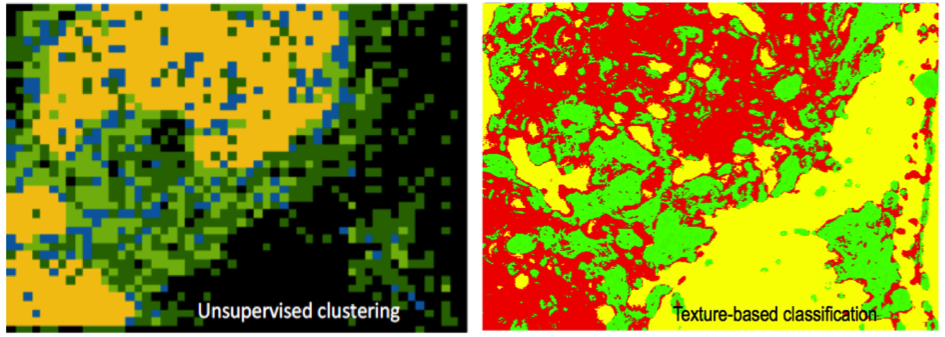
\includegraphics[width=0.85\textwidth]{figures/research/insitumrna.png}
\caption{\label{fig:carolina_insitu} Coupling gene expression to cell and tissue morphology. The gene expression map was divided into patches of $100\times100$ pixels, and patches were clustered by k-means clustering (100 random seeds). The resulting spatial patterns (left) correlate with independent texture-based classification (right) of an H\&E staining of the same tissue sample.} 
\end{figure}

% EEE

\item 
\textbf{Evaluation of the Effect of Compaction Oligonucleotides on the Strength and Integrity of Florescent Signals }\\
Omer Ishaq, Petter Ranefall, Carolina W\"{a}hlby\\
\ppartners{Carl-Magnus Clausson, Linda Andersson, Ola S\"{o}derberg, Dept.~of Immunology, Genetics and Pathology, UU}
\ffunding{SciLife Lab Uppsala}
\pperiod{1310--}
\aabstract{Rolling circle amplification (RCA) performs nucleic acid replication for rapid synthesis of multiple concatenated copies of circular DNA. These molecules can be visually observed through the use of florescent markers. Moreover, the introduction of a compaction oligonucleotide during RCA results in brighter and more compact signals. The project aims to evaluate the effect of compaction oligonucleotides on the strength and integrity of florescent signals. A manuscript has been submitted for journal publication.}






\item
\label{proj:stemcells}
\textbf{SciLifeLab Cancer Stem Cell Program}\\
Damian Matuszewski, Carolina W\"{a}hlby, Ida-Maria Sintorn\\
\ppartners{Sven Nelander, Karin Forsberg-Nilsson, Irina Alafuzoff, Ulf Landegren, Anna Segerman, Tobias Sj\"{o}blom, Lene Urborn and Bengt Westermark, Dept.~of Immunology, Genetics and Pathology and SciLifeLab, UU, Bo Lundgres, the Karolinska Institute and SciLifeLab, Stockholm, Rebecka J\"{o}rnsten, Chalmers, Gothenburg, and G\"{o}ran Hesselager, UU Hospital, Uppsala}
\ffunding{AstraZeneca-Science for Life Laboratory Joint Research Program}
\pperiod{1303--}
\aabstract{The SciLifeLab Cancer Stem Cell Program is a cross-platform initiative to characterize cancer stem cells (CSCs). Previously, the development of drugs targeting the CSC population in solid tumors has been curbed by the lack of valid cell model systems, and the complex genetic heterogeneity across tumors, factors that make it hard to assess new targets or predict drug responses in the individual patient. To solve these problems, our aim is to develop a biobank of highly characterized CSC cultures as a valid model of cancer heterogeneity. We will combine mathematical and experimental approaches, including image-based high-throughput cell screening, to define the spectrum of therapeutically relevant regulatory differences between patients. This will help elucidate mechanisms of action and enable accurate targeting of disease subgroups. During 2013-2014, patient data was collected, and a number of primary cell lines were established. Cultured cells were exposed to a different treatments and doses (more than 2500 different treatments per cell line), and imaged by fluorescence as well as bright-field microscopy, and current focus is on extracting meaningful morphological descriptors from the image data (Figure \ref{fig:stemcell}). 
Developed tools are also applied in a cell cycle analysis project realized together with Jordi Carreras Puigvert, the Karolinska Institute and SciLifeLab, Stockholm.}


\begin{figure}[!htbp]
	\centering
	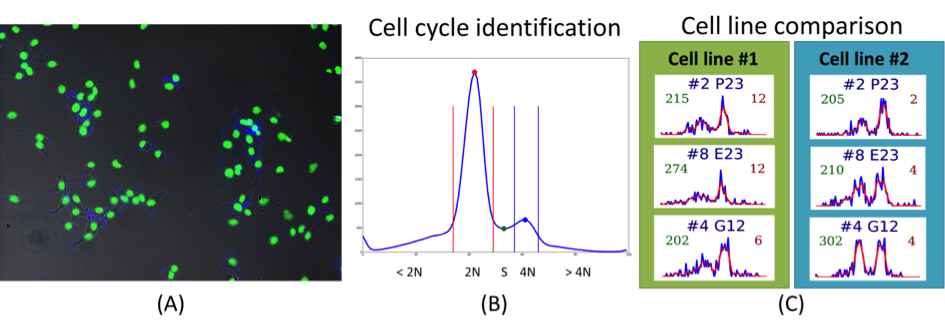
\includegraphics[width=0.85\textwidth]{figures/research/stemcell.png}
	\caption{(A) Sample cancer stem cells image. (B) and (C) present histograms of one of the automatically extracted features DNA content per cell. (B) The different phases of the cell cycle can be identified based on the DNA content in negative control cells, by assuming that cells spend the majority of their time with either two ($2N$ phase) or four ($4N$ phase) copies of the DNA. Cells from different cell lines respond in a slightly different way to the same drug treatments. (C) DNA histograms for treatments that arrest part of the cell population in the $4N$ phase.} 
	\label{fig:stemcell}
\end{figure}

%HHH

\item \textbf{Endothelial Cell Segmentation of the Cornea of Human Eyes}\\
Bettina Selig, Cris Luengo\\
\ppartners{Bernd Rieger, Quantitative Imaging Group, Delft University
of Technology, The Netherlands; Koen Vermeer, The Rotterdam Eye Hospital, The Netherlands}
\ffunding{S-faculty, SLU}
\pperiod{1103--1412}
\aabstract{The corneal endothelium plays a key role in maintaining the transparency of the cornea.Because the cells in the endothelium do not regenerate, the cell density decreases with age; this reduces its ability to maintain the processes needed to keep the cornea transparent. Thus, being able to measure this density in patients is very important. The endothelium can be imaged by specular microscopy or by confocal scanners, and measurements can be obtained manually, automatically with manual corrections, or fully automatically with current software (e.g., Nidek's NAVIS). Unfortunately, the results of the automatic methods are often useless, especially at low cell densities. Together with the Rotterdam Eye Hospital, we have developed a fully automatic method to segment individual cells in the corneal endothelium. The result of the method can be used to determine the cell density, but also other parameters of interest, like pleomorphism (cell shape) and polymegathism (cell size variation). Our segmentation method produces a segmentation that matches a manual segmentation reasonably well, for a wide range of cell densities and image qualities. These results have been submitted for publication during 2014.}



%%% III

\item \textbf{CerviScan}\\
Ewert Bengtsson, Patrik Malm, Bo Nordin\\
\ppartners{Rajesh Kumar, Centre for Development of Advanced Computing (CDAC), Thiruvananthapuram, Kerala, India; K. Sujathan, Regional Cancer Centre, Thiruvananthapuram, Kerala, India; Andrew Mehnert, Chalmers}
\ffunding{Swedish Governmental Agency for Innovation Systems (VINNOVA); Swedish Research Council; SIDA}
\pperiod{0801--}
\aabstract{Cervical cancer is a disease that annually kills over a quarter of a million women world-wide. This number could be substantially reduced if women were regularly screened for signs of cancer precursors using the well-established Pap-test. If detected early, these precursors can be treated with a very high rate of success. A problem with the Pap-test is that it requires highly trained cytotechnologists to perform the time consuming visual analysis of the specimen. For over 50 years attempts to automate this process have been made but still no cost effective systems are available.
	
The CerviScan project is an initiative from the Indian government, managed by the research institute CDAC in cooperation with the Regional Cancer Centre (RCC) in Kerala and CBA in Sweden, aimed at creating a low cost, automated screening system. The system will reduce the number of cytotechnologists needed for population screening by identifying and removing specimen that are clearly normal. A prototype system has been created and used to screen over 1000 specimen. Initial classification results are promising but screening times are still about 10 times longer than what is realistic in a real screening setting. Plans for the next phase of the project, focusing on dedicated hardware, are awaiting the result of a funding application in India.
 
A sub project on developing improved ways of describing the nuclear chromatin patterns based on new image analysis methods has been spun off and is describe as Project \ref{proj:high_prec_lifeSci}. The project has resulted in several recent publications. Patrik Malm defended his PhD thesis closely linked to this project in February 2014.}


\item 
\textbf{Automated Tissue Image Analysis using Pattern Recognition}\\
Jimmy Azar, Anders Hast, Ewert Bengtsson \\
\ffunding{TN-faculty, UU}
\pperiod{1001--1410}
\aabstract{The research was initially part of a VR supported project for grading of prostate cancer. The final part of the research which took place during 2014 extended this to more general ways of describing the architecture of histological tissues.
	 
Immunohistochemistry can facilitate the quantification of biomarkers such as estrogen, progesterone, and the human epidermal growth factor 2 receptors, in addition to Ki-67 proteins that are associated with cell growth and proliferation. We developed a method for the identification of paired antibodies based on correlating probability maps of immunostaining patterns across adjacent tissue sections. Samples from the Human Protein Atlas project were used to test the method.

We also developed a new feature descriptor for characterizing glandular structure and tissue architecture, which form an important component of Gleason and tubule-based Elston grading. The method is based on defining shape-preserving, neighborhood annuli around lumen regions. 

These two studies were accepted as journal papers. Jimmy Azar defended his PhD thesis closely linked to this project in October 2014.}


% NNN

\item 
\textbf{Segmentation and Tracking of E.coli Bacteria in Bright-Field Microscopy Images}\\
Sajith Kecheril Sadanandan, Carolina W\"{a}hlby\\
\ppartners{Johan Elf, David Fange, Alexis Boucharin, Dept.~of Cell \& Molecular Biology, UU; Klas E. G. Magnusson, Joakim Jald\'en, ACCESS Linnaeus Centre, KTH.}
\ffunding{SciLifeLab Uppsala, eSSENCE, VR junior researcher grant to CW}
\pperiod{1210--}
\aabstract{Live cell experiments pave way to understand the complex biological functions of living organisms. Most live cell experiments require monitoring of cells under different conditions over several generations. The biological experiments display wide variations even when performed under similar conditions, and therefore need to include large population studied over several generations to provide statistically verifiable conclusions. Time-lapse images of such experiments usually generate large quantities of data, which become extremely difficult for human observers to evaluate. Thus, automated systems are helpful to analysis of such data and provide valuable inference from the experiment. In this work we segment and track E. coli bacteria cells over time. We developed a novel segmentation method, which is fast and robust in delineating bacterial cells in phase contrast microscopy images. The preliminary results (Figure \ref{fig:ecoliseg}) were presented as poster at the International Bioimage Informatics 2014 conference in Leuven, Belgium.}

\begin{figure}[!htbp]
	\centering
	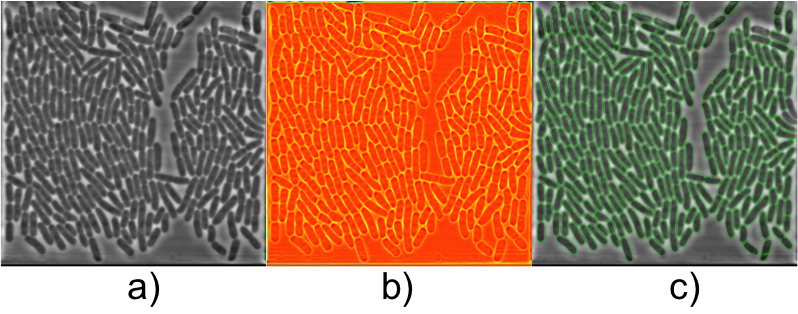
\includegraphics[width=0.85\textwidth]{figures/research/ecoliseg.png}
	\caption{a) Input phase contrast image of E. coli bacteria, b) contrast enhanced image and c) segmentation result overlaid on the input image.} 
	\label{fig:ecoliseg}
\end{figure}

%\newpage

%OOO

\item % Analysis of microscopic biomedical images
\label{proj:cellsurfaceDiffusion}
\textbf{Modelling Diffusion on Cell Surfaces}\\
Ida-Maria Sintorn, Robin Strand \\
\ppartners{Ingela Parmryd, Dept.~of Medical Cell Biology, UU; Jeremy Adler, Dept.~of Immunology, Genetics and Pathology, UU}
\ffunding{TN-faculty, UU; S-faculty, SLU; VINNMER programme, Swedish Governmental Agency for Innovation Systems}
\pperiod{1101--}
\aabstract{A cell surface is a highly irregular and rough. The surface topography is however usually ignored in current models of the
	plasma membrane, which are based on 2D observations of diffusion that really occurs in 3D. In this project, we model diffusion on
	non-flat surfaces to explain biological processes occurring on the cell surface. }

%PPP

\item 
\textbf{Analysis of Male Reproductive Tract Morphology in Reproductive Toxicology}\\
Azadeh Fakhrzadeh, Cris Luengo, Gunilla Borgefors\\
\ppartners{Ellinor Sp\"{o}rndly-Nees,  Lena Holm, Dept.~of Anatomy, Physiology and Biochemistry, SLU}
\ffunding{SLU (KoN)}
\pperiod{1009--}
\aabstract{Reproductive toxicology is the study of chemicals and their effects on the reproductive system of humans and animals. In reproductive toxicology, there is a strong need to detect structural differences in organs that often have both a complex microscopic structure and function. This problem is further complicated because standard techniques are based on the examination of two-dimensional sections of a three-dimensional structure. The aim of this project is to develop methods to objectively describe microscopic structures of male reproductive organs and to test these in reproductive toxicology research. The project is comparative and includes studies of organs from rooster and mink. We are developing automatic and interactive methods to analyse the relevant structures in the histology images of testis.

Generating sperm in seminiferous tubules is a cyclic process, during which various generations of germ cells in the epithelial layer undergo a series of developmental steps. This cycle is typically subdivided into 12 different stages. We are developing a texture-based classification method to determine each tubule's stage. We are able to distinguish consistently stages if they are grouped into five classes (Figure \ref{fig:malereprod}).}

\begin{figure}[h]
\centering %\scalebox{1}{}
\includegraphics[width=0.8\textwidth]{figures/research/5class.pdf}
 \caption{Cross sections of seminiferous tubules representative for	the five classes we can distinguish consistently. Differences are mostly in the shape of the nuclei (stained in brown).}
 \label{fig:malereprod}
 \end{figure}

%\newpage
%RRR

\item % Analysis of microscopic biomedical images
\label{proj:CombatingCancer}
\textbf{Combating Breast Cancer by Digital Pathology}\\
Andreas K{\aa}rsn\"{a}s, Robin Strand, Carolina W\"{a}hlby, Ewert Bengtsson\\
\ppartners{Visiopharm, H{\o}rsholm, Denmark; Clinical Pathology Division, Vejle Hospital, Vejle, Denmark}
\ffunding{NordForsk Private Public Partnership PhD Programme and Visiopharm}
\pperiod{0909--1412}
\aabstract{The results of analyses of tissue biopsies by pathologists are crucial for breast cancer patients. In particular, the precision of a patient's prognosis, and the ability to predict the consequences of various treatment opportunities before actually exposing the cancer patient, depend on the detection and quantification of biomarkers in tissue sections by microscopy. Experience from the last decade has revealed that manual detection and quantification of biomarkers by microscopy of tissue biopsies is highly dependent on the competencies and stamina of the individual pathologist. The aim of the present PhD project is to develop software-based algorithms that can facilitate the workflow and ensure objective and more precise results of the quantitative microscopy procedures in breast cancer.
	
Andreas K{\aa}rsn\"{a}s defended his PhD thesis closely linked to this project in April 2014. A manuscript describing a new method for registering histological images of consecutive sections with different staining by using locally rigid transforms is currently under review and a journal article presenting a histopathological tool for sub-cellular quantification was accepted for publication in the journal \textit{Computer methods in Biomechanics and Biomedical Engineering: Imaging \& Visualization}, in 2014}

%SSS

\item 
\textbf{Automatic, Quantitative Malignancy Grading of Prostate Cancer using Image Analysis}\\
Ingrid Carlbom, Christophe Avenel\\
\ppartners{Christer Busch, Department of Surgical Sciences, and Anna Tolf, Department of Genetics and Pathology, University Hospital}
\ffunding{The Swedish Research Council; Hagstrandska fonden.}
\pperiod{1001--}
\aabstract{\textit{Online Prostate Tissue Grading Tool: }Using our OpenSeaDragon-based image selection tool we built an image database of 650 small images from whole mount sections, where each image has one dominant pattern that represents a malignancy grade, precancerous tissue, or benign tissue. With our online grading tool, fourteen internationally prominent pathologists from seven countries are in the process of grading these images according to the Gleason system (Figure \ref{fig:userintpros}). 
	
With 50\% of the images graded, we see similar grade variations as seen in other studies; for example, in 43\% of the cases more than three pathologists disagree. But unlike other studies on intra- and interobserver grading variation, which are based on entire biopsies or whole mounts, each image in our study contains only one dominant pattern, allowing us to identify patterns that cause the discrepancies. Our goal is to establish a consensus for these patterns, thereby promoting international grading standardization.

\textit{Automatic segmentation of prostate glands and nuclei: }Using the stromal density map from the color decomposition of Sirius-hematoxylin-stained tissue, we extract the glandular structures using morphological operations combined with standard image processing operations. With the glandular units as masks, we then extract the epithelium and the lumen from the epithelial density maps. Qualitative analysis of over 5000 glands indicates that the segmentation results in highly accurate representations of the glandular shape, including the epithelium and the lumen (Figure \ref{fig:segglandpros}a).

Earlier we developed an algorithm to find the epithelial nuclei locations and approximate shapes in the epithelial density maps. We have augmented the algorithm to find a more precise shape of the nuclei using a deformable circular model (Figure \ref{fig:segglandpros}b).

\textit{Consensus-Based Training Dataset: }	Using the automatically segmented glandular units, we label each gland based on the Gleason Grade produced by one pathologist. This labelling is on a finer scale than the Gleason grades; for example, grade 4 will be separated into fine caliber 4 and cribriform 4. Other grades are also divided to capture differences within the grade. To date we have labelled more than 5000 glands with one pathologist, giving us a dataset for continued development of our automatic grading algorithm. The labels will be updated when we reach a consensus grade with our international panel of experts.}

\begin{figure}[!htbp]
	\centering
	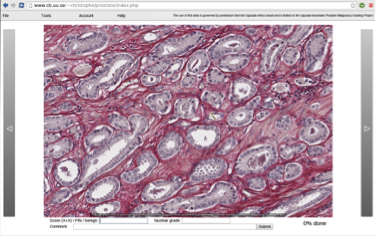
\includegraphics[width=.6\textwidth]{figures/research/userinterfaceprostate.png}
	\caption{The user gives a Gleason Score below the image or indicate PIN or benign as the primary pattern} 
	\label{fig:userintpros}
\end{figure}

\begin{figure}[!htbp]
	\centering
	\subfigure[]{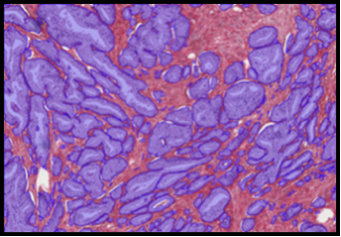
\includegraphics[width=0.4\textwidth]{figures/research/segglandpros.png}}
	\subfigure[]{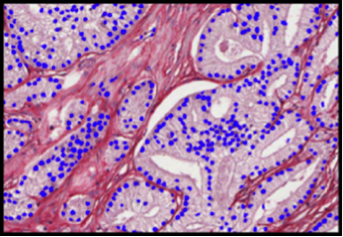
\includegraphics[width=0.4\textwidth]{figures/research/segnucleipros.png}}
	\caption{(a) Segmented glands; (b) Segmented epithelial nuclei}
	\label{fig:segglandpros}
\end{figure}


%TTT
\newpage


%UUU

\item 
\textbf{Quantification of Zebrafish Lipid Droplets}\\
Petter Ranefall, Carolina W\"{a}hlby\\
\ppartners{Marcel den Hoed, Manoj Bandaru, Erik Ingelsson, Dept.~of Medical Sciences and SciLifeLab, UU}
\ffunding{SciLifeLab Uppsala}
\pperiod{1308--}
\aabstract{The aim of this project is to identify novel targets for the therapeutic intervention of coronary artery disease. This is done by following-up results from genome-wide association studies in epidemiological studies using a zebrafish model system. Using image analysis we try to identify and characterize causal genes within loci that have so far been identified as associated with coronary heart disease by (high-throughput) screening of atherogenic processes in wildtype and mutant zebrafish, both before and after feeding on a control diet or a diet high in cholesterol. Using confocal microscopy we can image fat accumulation in the zebrafish. Our results confirm that zebrafish larvae represent a promising model system for early-stage atherosclerosis. An abstract has been submitted.}



% XXX

\item
\label{proj:gigapixel}
\textbf{Tools for Analysis and Visualization of Giga-Pixel Sized  Slide-Scanner Images.}\\
Petter Ranefall, Alexandra Pacureanu, Carolina W\"{a}hlby, Thu Tran\\
\ppartners{Mats Nilsson, Thomas Hauling, Marco Mignardi, Jessica Svedlund, Elin Lundin, Xiaoyan Qian, Dept.~of Biochemistry and Biophysics and SciLifeLab, Stockholm University.}
\ffunding{SciLifeLab}
\pperiod{1308--}
\aabstract{The aim is to create a tool for full resolution image analysis of large images, e.g. slide scanner data, with the possibility of visual examination and interaction at multiple resolutions. The tool is built on a free and open-source framework for visual examination at multiple resolutions with the option to toggle results on or off, such as segmentation masks, classification results, and tissue morphology measurements, using a map view with seamless zooming and panning capabilities, allowing for fast navigation between a full-tissue view and high-resolution sub-cellular observations. The aim is to also have an interface that enables visual/manual selection of regions of interest, target discovery, and understanding of novel spatial relationships within the tissue environment. A bachelor thesis project with the aim of designing the user interface was carried out by the student Thu Tran. This user interface has then been extended with full functionality into a system that we call 'TissueMaps', which is now being evaluated at Mats Nilsson's lab. During 2014 'TissueMaps' has also been presented/demonstrated at some different conferences: BioImage Informatics in Leuven, Belgium, eSSENCE in Ume\aa, SSBA in Lule\aa, and the Nordic Symposium on Digital Pathology in Link\"oping.}

%%%

\item
\label{proj:high_prec_lifeSci}
\textbf{Advanced Methods for Reliable and Cost Efficient Image Processing in Life Sciences}\\
Nata\v{s}a Sladoje, Ewert Bengtsson,  Ida-Maria Sintorn  \\
\ppartners{Joakim Lindblad, Faculty of Technical Sciences, University of Novi Sad, Serbia}
\ffunding{Swedish Governmental Agency for Innovation Systems (VINNOVA); UU TN-faculty }
\pperiod{1308--}
\aabstract{Within this project we aim at advancing the state-of-the-art methods of digital image processing and analysis, so that some of the societally important and highly challenging and relevant research task in life sciences can be successfully addressed.  Our goal is to increase reliability and efficiency, as well as robustness against variations in preparation quality, of computer assisted image analysis in two particular research tracks, related to two applications: (1) Chromatin distribution analysis for cervical cancer diagnostics, and (2) virus detection and recognition in TEM images. 
	
Advances in cyto-patological research combined with the desire for as early as possible cancer detection, have put focus on the analysis of very subtle changes in the chromatin structure of cell nuclei. The application related to recognition and classification of viruses	is focused on development of efficient methods adjusted to less expensive equipment, by that increasing applicability and usefulness of the results for a wider community. Efficient utilization of available images data to characterize barely resolved structures, is crucial in both cases. The intention is to use results from resent theoretical work within the framework of discrete mathematics, where  knowledge from the field of fuzzy sets is combined with explicit usage of intensity and shape information in images. This theoretical framework provides methods which enable preservation and efficient usage of information, aggregate information of different types, improve robustness of the developed methods and increase precision of the analysis results. Based on conducted studies, the developed framework has shown high potential in applications where efficient utilization of information is of importance and where reliability of the analysis results and their timely delivery are both required. }

\clearpage

\subsection{3D analysis and visualization}

%AAA

\item 
\label{proj:CMS}
\textbf{Haptics and its Applications to Medicine}\\
Ingrid Carlbom, Pontus Olsson, Fredrik Nysj\"{o}\\
\ppartners{Stefan Johansson (Division of Microsystems Technology, UU and Teknovest AB); Jan-Micha{\'e}l Hirsch, Dept.~of Surgical Sciences, Oral \& Maxillofacial Surgery, UU and Consultant at Dept.~of Plastic- and Maxillofacial Surgery, UU Hospital; Andreas Thor, Dept.~of Surgical Sciences, Oral \& Maxillofacial Surgery, UU Hospital; Andres Rodriguez Lorenzo, Dept.~of Surgical Sciences, Plastic Surgery, UU Hospital; PiezoMotors AB.}
\ffunding{Dept.~of Surgical Sciences, Oral \& Maxillofacial Surgery, UU Hospital; Thur\' eus Stiftelsen}
\pperiod{1301--}
\aabstract{This year we augmented the Uppsala Haptics-Assisted Surgery Planning (UHASP) system with virtual reconstruction of head and neck defects by fibula osteocutaneous free flaps (FOFF), including bone, vessels, and soft-tissue of the FOFF in the defect reconstruction. With the UHASP stereo graphics and haptic feedback, using patient-specific CT-angio data, the surgeons can plan bone resection, fibula design, recipient vessels selection, pedicle and perforator location selection, and skin-paddle configuration.

Two surgeons tested UHASP on four cases they had previously operated: three with composite mandibular defects and one with a composite cervical spine defect (Figure \ref{fig::haptics}). During the planning session, it became apparent that some problems encountered during the actual surgery could have been avoided. In one case, the fibula reconstruction was incomplete since the fibula had to be reversed and thus did not reach the temporal fossa. In another case, the fibula had to be rotated 180 degrees to correct the plate and screw placement in relation to the perforator. In the spinal case, difficulty in finding the optimal fibula shape and position required extra ischemia time. The surgeons found UHASP to be an efficient planning tool for FOFF reconstructions. The testing of alternative reconstructions to arrive at an optimal FOFF solution preoperatively potentially improves patient healing, function and aesthetics, and reduces operating room time.}

\begin{figure*}[!htbp]
\centering
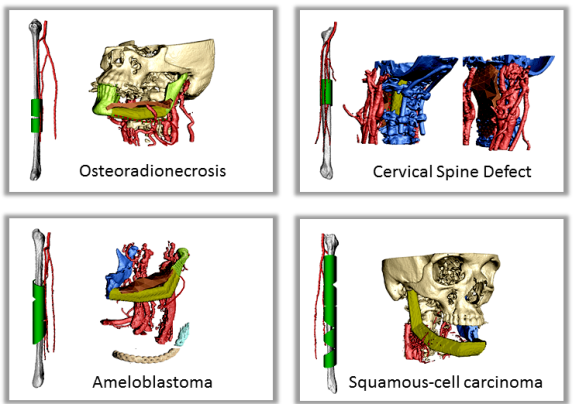
\includegraphics[width=0.9\textwidth]{figures/research/haptics.png}
\caption{The resulting plans for the four cases. The whole fibula with osteotomy positions and orientations are shown in relation to
surrounding vessels to the left of each case.}
\label{fig::haptics}
\end{figure*}


\item 
\textbf{ProViz -- Interactive Visualization of 3D Protein Images}\\
Lennart Svensson, Ida-Maria Sintorn, Ingela Nystr\"{o}m, Fredrik Nysj\"{o}, Johan Nysj\"{o}, Anders Brun, Gunilla Borgefors\\
\ppartners{Dept.~of Cell and Molecular Biology, Karolinska Institute; SenseGraphics AB}
\ffunding{The Visualization Program by Knowledge Foundation; Vaardal Foundation; Foundation for Strategic Research; VINNOVA; Invest in Sweden Agency; SLU, faculty funding}
\pperiod{0807--1412}
\aabstract{Electron tomography is the only microscopy technique that allows 3-D imaging of biological samples at nano-meter resolution. It thus enables studies of both the dynamics of proteins and individual macromolecular structures in tissue. However, the electron tomography images have a low signal-to-noise ratio, which makes image analysis methods an important tool in interpreting the images. The ProViz project aims at developing visualization and analysis methods in this area.

The project focus 2014 has been on finalizing and testing the methods and software as well as preparing the manuscript describing and demonstrating the ProViz software. Lennart Svensson defended his PhD thesis very closely linked to this project.}

% CCC
\item 
\label{proj:MRI_optimal_lattices}
\textbf{Analysis and Processing of Three-Dimensional Magnetic Resonance Images on Optimal Lattices} \\
Elisabeth Linn\'{e}r, Robin Strand\\
%ppartner{Joel Kullberg, Dept.~of Radiology, Oncology and Radiation Science, UU}
\ffunding{TN-faculty, UU}
\pperiod{1005--}
\aabstract{Three-dimensional images are widely used in, for example, health care. With optimal sampling lattices, the amount of data can be reduced by 20-30\% without affecting the image quality, lowering the demands on the hardware used to store and process the images, and reducing processing time.

In this project, methods for image acquisition, analysis and visualization using optimal sampling lattices are studied and developed, with special focus on medical applications. The intention is that this project will lead to faster and better processing of images with less demands on data storage capacity. One of the goals of the project is to release open source software for producing, processing, analyzing and visualizing volume images sampled on BCC and FCC lattices, so as to make them readily available for potential users to explore on their own.
During 2014, the focus has been on distance transforms. Two reviewed conference papers exploring a graph-based implementation of the anti-aliased Euclidean distance transform have been published, and the work on the open source software is progressing.}

% DDD

\item 
\label{proj:MRI_registration}
\textbf{Registration of Medical Volume Images}\\
Robin Strand, Filip Malmberg\\
\ppartner{Joel Kullberg, H{\aa}kan Ahlstr\"{o}m, Dept.~of Radiology, Oncology and Radiation Science, UU}
\ffunding{Faculty of Medicine, UU}
\pperiod{1208--}
\aabstract{In this project, we mainly process magnetic resonance tomography (MR) images. MR images are very useful in clinical use and in medical research, e.g., for analyzing the composition of the human body. At the division of Radiology, UU, a huge amount of MR data, including whole body MR images is acquired for research on the connection between the composition of the human body and disease.

To compare volume images voxel by voxel, we develop image registration methods. For example, large scale analysis is enabled by image registration methods that utilizes, for example, segmented tissue (e.g., Project~\ref{project:medical_segmentation}) and anatomical landmarks. Based on this idea, we have developed Imiomics (imaging omics) -- an image analysis concept, including image registration, that allows statistical and holistic analysis of whole-body image data (Figure \ref{fig:imiomics}). The Imiomics concept is holistic in three respects: (i) The whole body is analyzed, (ii) All collected image data is used in the analysis and (iii) It allows integration of all other collected non-imaging patient information in the analysis.}

\begin{figure*}[!htbp]
\centering
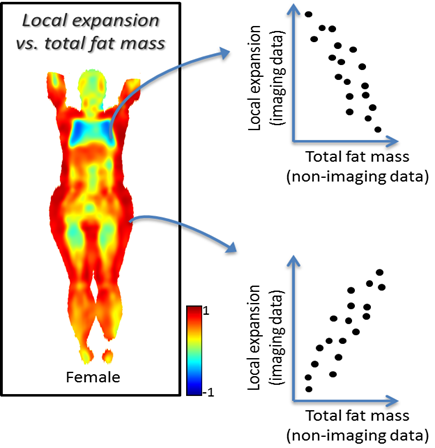
\includegraphics[width=0.6\textwidth]{figures/research/Imiomics_example.png}
\caption{\label{fig:imiomics} An illustration of a correlation map obtained by Imiomics. In this example, point-wise correlations between local tissue volume and body fat mass (measured by bioelectrical impedance analysis, BIA).} 
\end{figure*}

% EEE
\item 
\label{project:medical_segmentation}
\textbf{Interactive Segmentation and Analysis of Medical Images}\\
Filip Malmberg, Robin Strand, Ingela Nystr\"{o}m, Ewert Bengtsson\\
\ppartners{Joel Kullberg, H{\aa}kan Ahlstr\"{o}m, Dept.~of Radiology, Oncology and Radiation Science, UU}
\ffunding{TN-faculty, UU}
\period 1106--\\
\aabstract{Three-dimensional imaging technique such as computed tomography (CT) and magnetic resonance imaging (MRI ) are now routinely used in medicine. This has lead to an ever increasing flow of high-resolution, high-dimensional, image data that needs to be qualitatively and quantitatively analyzed. Typically, this analysis requires accurate segmentation of the image. 

At CBA, we have been developing powerful new methods for interactive image segmentation. In this project, We seek to employ these methods for segmentation of medical images, in collaboration with the Dept.~of Radiology, Oncology and Radiation Science (ROS) at the UU Hospital. 

During 2014, we published an article describing \emph{Smartpaint}, a tool for interactive segmentation of volume images. The SmartPaint software is publicly available and can be downloaded from \url{http://www.cb.uu.se/~filip/SmartPaint/}. To date, this software has been downloaded more than 500 times.} 

\item
\label{project:orbit_segmentation}
\textbf{Orbit Segmentation for Cranio-Maxillofacial Surgery Planning}\\
Johan Nysj\"{o}, Ida-Maria Sintorn, Ingela Nystr{\"o}m, Filip Malmberg\\
\ppartners{Jan Michael Hirsch, Andreas Thor, Johanna Nilsson, Dept.~of Surgical Sciences, UU Hospital; Roman Khonsari, Pitie Salpetriere Hospital, Paris, France; Jonathan Britto, Great Ormond Street Hospital, London, UK}
\ffunding{TN-faculty, UU}
\pperiod{0912--}
\aabstract{An important component in cranio-maxillofacial (CMF) surgery planning is to be able to accurately measure the extent of certain anatomical structures. The shape and volume of the orbits (eye sockets) are of particular interest. These properties can be measured in CT images of the skull, but this requires accurate segmentation of the orbits. Today, segmentation is usually performed by manual tracing of the orbit in a large number of slices of the CT image. This task is very time-consuming, and sensitive to operator errors. Semi-automatic segmentation methods could reduce the required operator time substantially. In this project, we are developing a prototype of a semi-automatic system for segmenting the orbit in CT images. The segmentation system is based on WISH, a software package for interactive visualization and segmentation that has been developed at CBA since 2003. WISH has been released under an open-source license and is available for download at \url{http://www.cb.uu.se/research/haptics}.

Our main focus during 2014 has been to continue our collaboration with surgeons from the Craniofacial Centre at Great Ormond Street Hospital, London, UK, in a project that aims to analyse the size and shape of the orbits in a large set of pre- and post-operative CT images of patients with congenital disorders. Our semi-automatic segmentation system has been used to rapidly segment the orbits in these datasets, and we have extended the system with automatic registration-based techniques for performing size and shape analysis of the segmented orbits. Abstracts about the ongoing work have been presented at medical conferences. We completed the size and shape analysis experiments for the study during the autumn and have now started to summarize the results in manuscripts.}

% GGG

\item 
\label{project:wrist_angle_measurements}
\textbf{Precise 3D Angle Measurements in CT Wrist Images}\\
Johan Nysj{\"o}, Filip Malmberg, Ingela Nystr{\"o}m, Ida-Maria Sintorn\\
\ppartners{Albert Christersson, Sune Larsson, Dept.~of Orthopedics, UU Hospital}
\ffunding{TN-faculty, UU}
\pperiod{1111--}
\aabstract{To be able to decide the correct treatment of a fracture, orthopedic surgeons need to assess the details about the fracture. One of the most important factors is the fracture displacement, particularly the angulation of the fracture. The wrist is the most common location for fractures in the human being. When a fracture is located close to a joint, for example, in the wrist,  the angulation of the joint line in relation to the long axis of the long bone needs to be measured. Since the surface of the joint line in the wrist is highly irregular, and since it is difficult to take X-rays of the wrist in exactly the same projections from time to time, conventional X-ray is not an optimal method for this purpose. In most clinical cases, conventional 2D angle measurements in X-ray images are satisfactory for making correct decisions about treatment, but when comparing two different methods of treatment, for instance, two different operation techniques, the accuracy and precision of the angle measurements need to be higher.

In this project, we are developing a system for performing precise 3D angle measurements in computed tomography (CT) images of the wrist. Our proposed system is semi-automatic; the user is required to guide the system by indicating the approximate position and orientation of various parts of the radius bone. This information is subsequently used as input to an automatic algorithm that makes precise angle measurements. We have developed a RANSAC-based method for estimating the long axis of the radius bone and a registration-based method (Figure \ref{fig:wrist}) for measuring the orientation of the joint surface of the radius. Preliminary evaluations have shown that these two methods together enable relative measurements of the dorsal angle in the wrist with sub-millimeter precision. During 2014, we performed a more extensive case study (involving 40 CT scan sequences of fractures wrists) to further evaluate the performance of our 3D angle measurement method and compare it with the conventional 2D X-ray measurement method. A manuscript about this study is under preparation.}

\begin{figure}[!htbp]
\centering
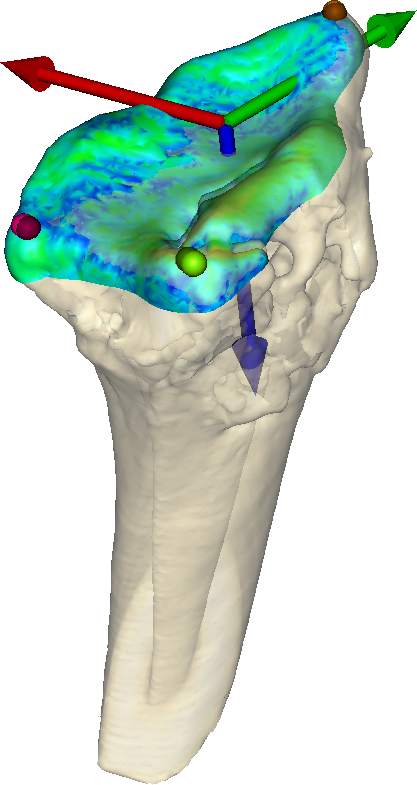
\includegraphics[height=0.9\textwidth, angle=90]{figures/research/wrist_2014.png}
\caption{\label{fig:wrist} Registration-based method for estimating the joint surface orientation in a fractured radius bone in the wrist. A template model of the joint surface is fitted to the target radius bone through landmark-guided surface registration, so that a local reference coordinate system of the template can be used to represent the joint surface orientation. The distance between the template and the joint surface is color-coded during the semi-automatic registration process.}
\end{figure}


% HHH

\item 
\textbf{Skeleton-Based Vascular Segmentation at Interactive Speed} \\
Krist\'{i}na Lidayov\'{a}, Hans Frimmel, Ewert Bengtsson \\
\ppartners{ \"{O}rjan Smedby, Chunliang Wang, Center for Medical Image Science and Visualization (CMIV), Link\"{o}ping University}
\ffunding{VR grant to \"{O}rjan Smedby}
\pperiod{1207--}
\aabstract{Precise segmentation of vascular structures is crucial for studying the effect of stenoses on arterial blood flow. The goal of this project is to develop and evaluate vascular segmentation, which will be fast enough to permit interactive clinical use. The first part is the extraction of the centerline tree (skeleton) from the gray-scale CT image. Later this skeleton is used as a seed region. The method should offer sub-voxel accuracy. 
	
	During 2013, we improved the software for fast vessel centerline tree extraction. The method has been tested on several CT data and the results look promissing. Generally main vessel centerlines are detected, but an improvement  needs to be done in order to remove some false positive centerlines. 
	
	In year 2014, we improved the software to its final stage. It works on the original Computed Tomography Angiography (CTA) image as the input and produces a node-link representation of the vascular structures for the lower limbs. The method (Figure \ref{fig:krstinapipeline}) works in two passes: first pass extracts the skeleton of large arteries, and second pass focus on extracting small arteries. Each pass contains three major steps: (1) sets proper intensity ranges for different anatomy structures based on Gaussian curve fitting to the image histogram; (2) apply different filters to detect voxels that are part of arteries, where filters are designed based on intensity and size analysis of ellipse shape on 2-D planes; (3) connect nodes to obtain a centerline tree for the entire vasculature. The method has been tested on 25 CTA scans of the lower limbs (Figure \ref{fig:krstinacomparison}) and achieved an average of 96\% overlap rate with ground truth. The average computational time is 121 sec/scan.
	
	A paper summarizing this work was written and was sent to a Special issue of Pattern Recognition Letters on skeletonization and its applications. At the current stage the paper is under major revision. The work was pressented at SSBA conference and Medicinteknikdagarna.}

\begin{figure}[!htbp]
	\centering
	\includegraphics[width=0.7\textwidth]{figures/research/kristinapipeline.pdf}
	\caption{Flow chart of the proposed method}
	\label{fig:krstinapipeline} 
	
\end{figure}

\begin{figure}[!htbp]
	\centering
	\includegraphics[width=0.7\textwidth]{figures/research/LiverSegBoundary3.pdf}
	\caption{Maximum intensity projection, resulting skeleton in red colour and reference skeleton in blue colour are shown for two cases from a clinical routine, (a) contains an occluded segment in the femoral artery, (b) contains an arterial stent.} 
	\label{fig:krstinacomparison}
\end{figure}


\item
\label{proj:feione}
\textbf{Ubiquitous Visualization in the Built Environment}\\
Stefan Seipel, Fei Liu\\
\ppartner{Dept.~of Industrial Development, IT and Land Management, University of G\"{a}vle}
\ffunding{University of G\"{a}vle; TN-faculty, UU}
\pperiod{1108--}
\aabstract{ This project deals with mobile visualization and augmented reality (AR) in indoor and outdoor environments. Several key problems for robust mobile visualization are addressed such as spatial tracking and calibration; image based 2D and 3D registration and efficient graphical representations in mobile user interfaces.

During 2014, two major lines of work have been carried out: Registration of thermal infrared and visible facade images for augmented reality-based building inspection. Here, the problem of multi-modal image registration is addressed through identification of high-level (quadrilateral) features which model the shapes of commonly present facade elements, such as windows (Figure \ref{fig:regone}). These features are generated by grouping edge line segments with the help of image perspective information, namely, vanishing points. Our method adopts a forward selection algorithm for selecting feature correspondences needed to estimate the transformation model (Figure \ref{fig:regtwo}). During the formation of the feature correspondence set, the correctness of selected feature correspondences at each step is verified through the quality of the resulting registration, which is based on the ratio of areas between the transformed features and the reference features. Part of this work has been published in the Journal of Image and Graphics. Other results of this work are currently prepared for publication.}

\begin{figure}[!htbp]
\centering
\includegraphics[width=0.6\textwidth]{figures/research/features.pdf}
\caption{\label{fig:regone} Selected control points for registration. Within an image, control points with the same color means they are from the same quadrilateral feature while across the images, the same color indicates correspondence.} 
\end{figure}

\begin{figure}[!htbp]
\centering
\includegraphics[width=0.5\textwidth]{figures/research/regiresult.pdf}
\caption{\label{fig:regtwo} Registration result showing the fusion of thermal infrared and visible images by alpha blending.} 
\end{figure}

Another activity in the project has been the development of a video-see through augmented reality system along with an experimental study on positioning accuracy in indoor augmented reality. In this work, a marker-based augmented reality application has been developed which displays construction elements (pipes) hidden inside walls as virtual models that are visually overlaid in real time upon video images of the real wall (Figure \ref{fig:arcomp}). Using this application, we conducted a user experiment to find out how precise the localization of hidden structures in walls could be performed by the use of a video-see through augmented reality guidance system. Another objective was to investigate different factors that are influential on positioning accuracy, such as e.g. visual parallax and method for targeting (Figure \ref{fig:arlab}). Experiment results have been gathered and as of now they are analyzed and prepared for publication. 

\begin{figure}[!hbp]
\centering
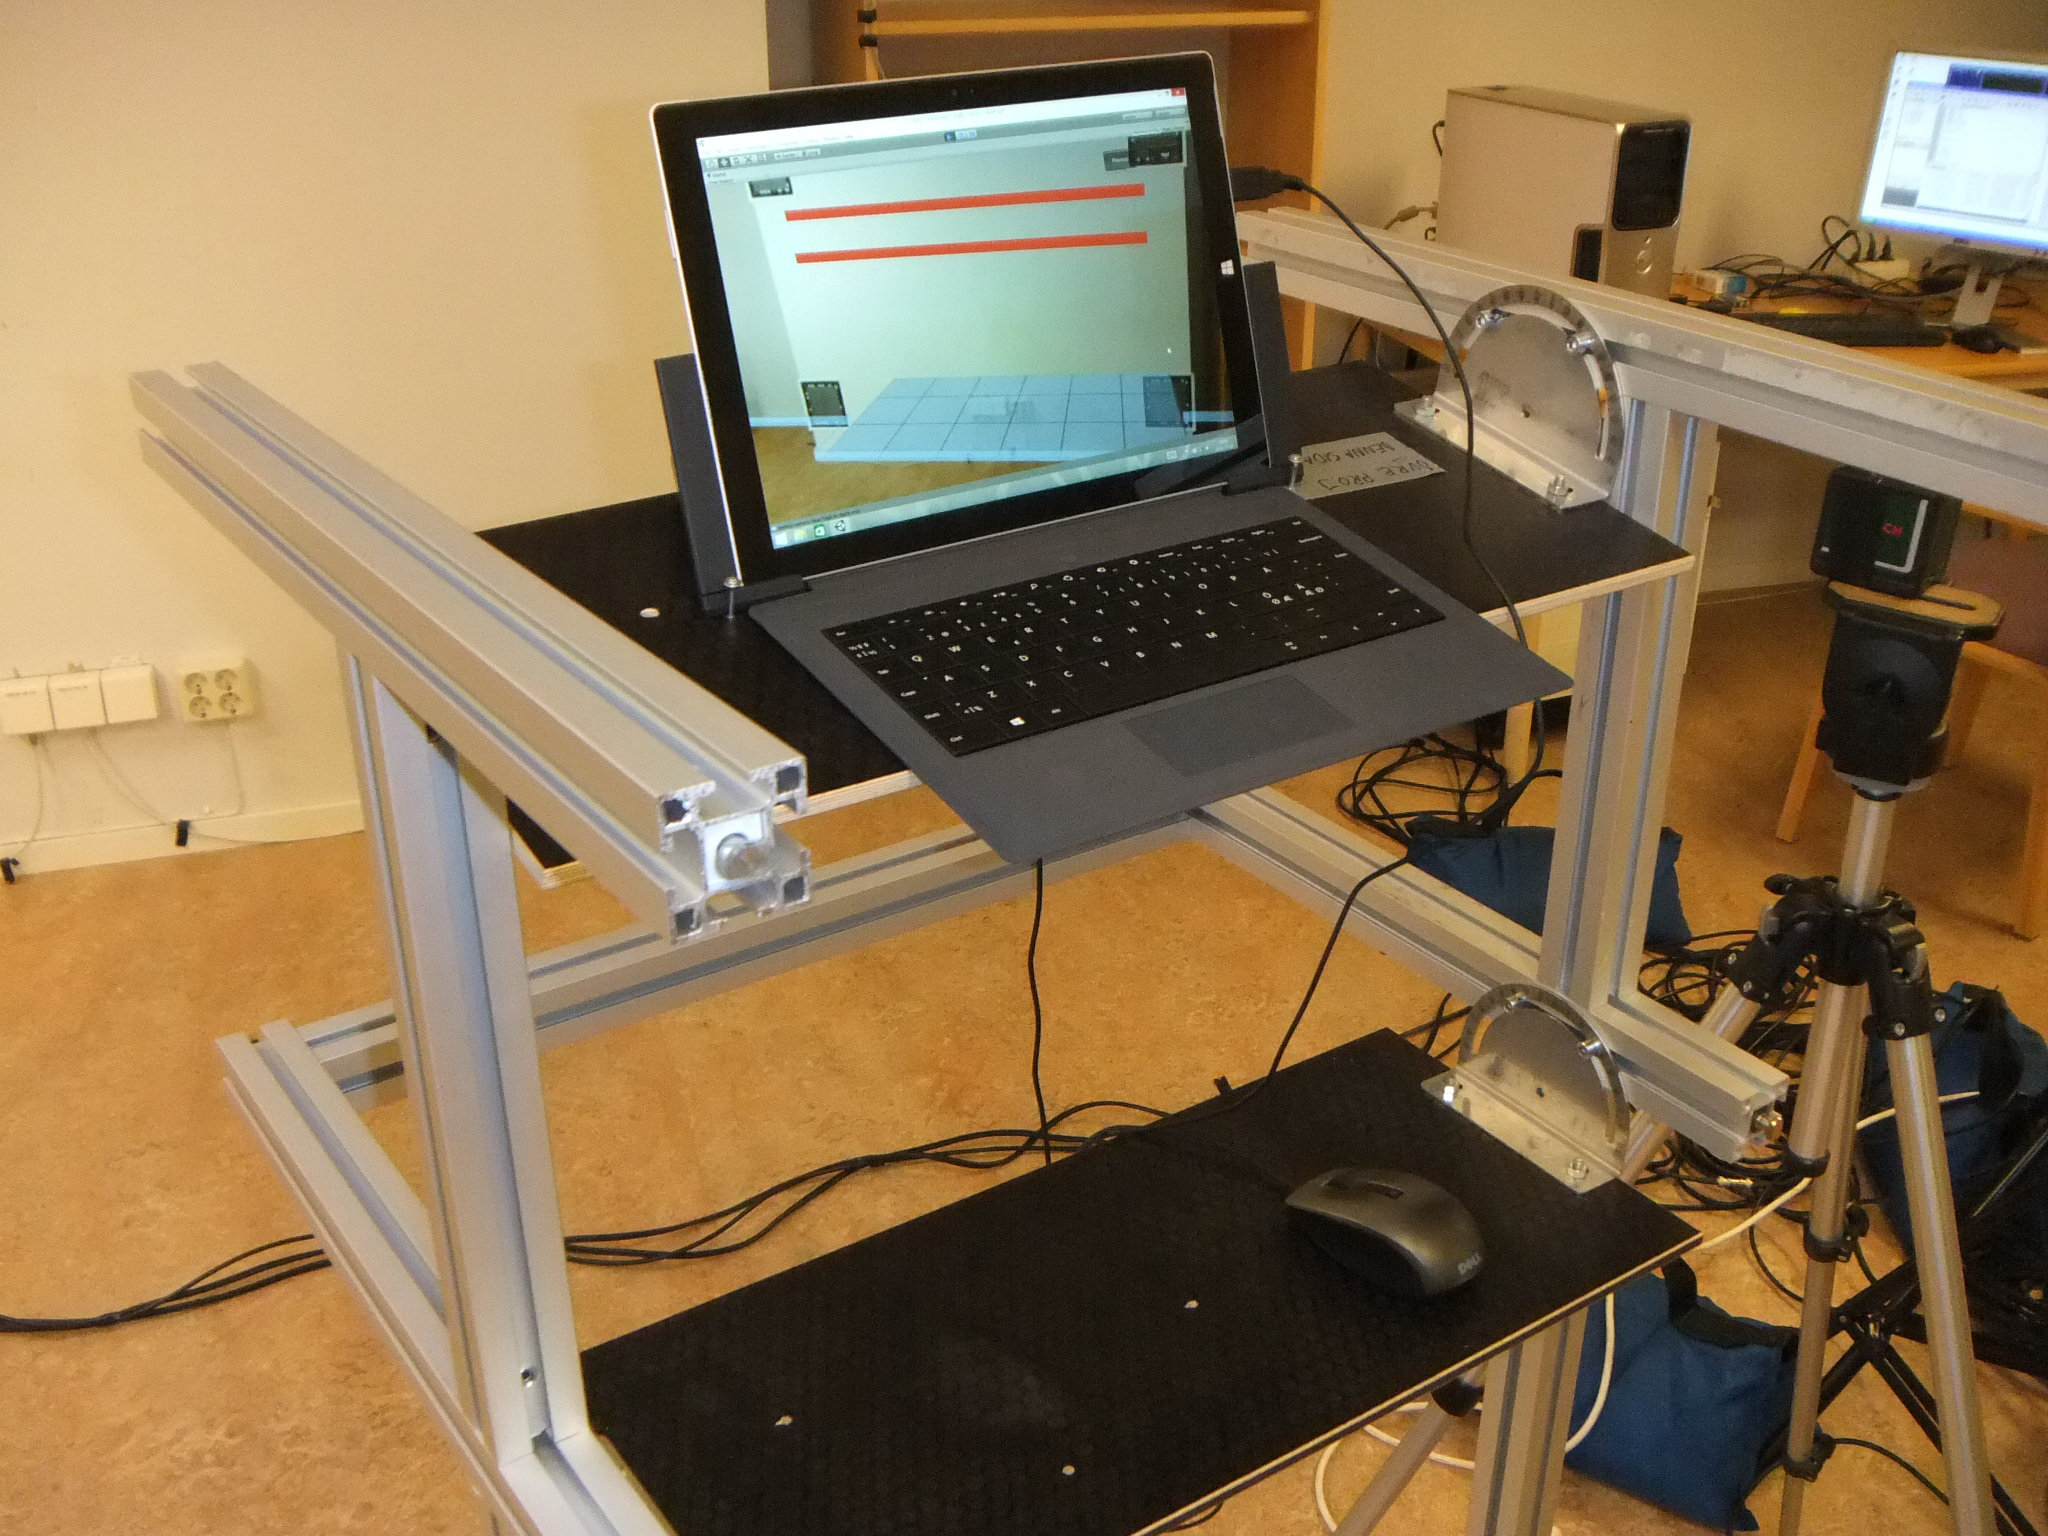
\includegraphics[width=0.6\textwidth]{figures/research/arapp.jpg}
\caption{\label{fig:arcomp} The augmented reality application running on the tablet.} 
\end{figure}

\begin{figure}[!hbp]
\centering
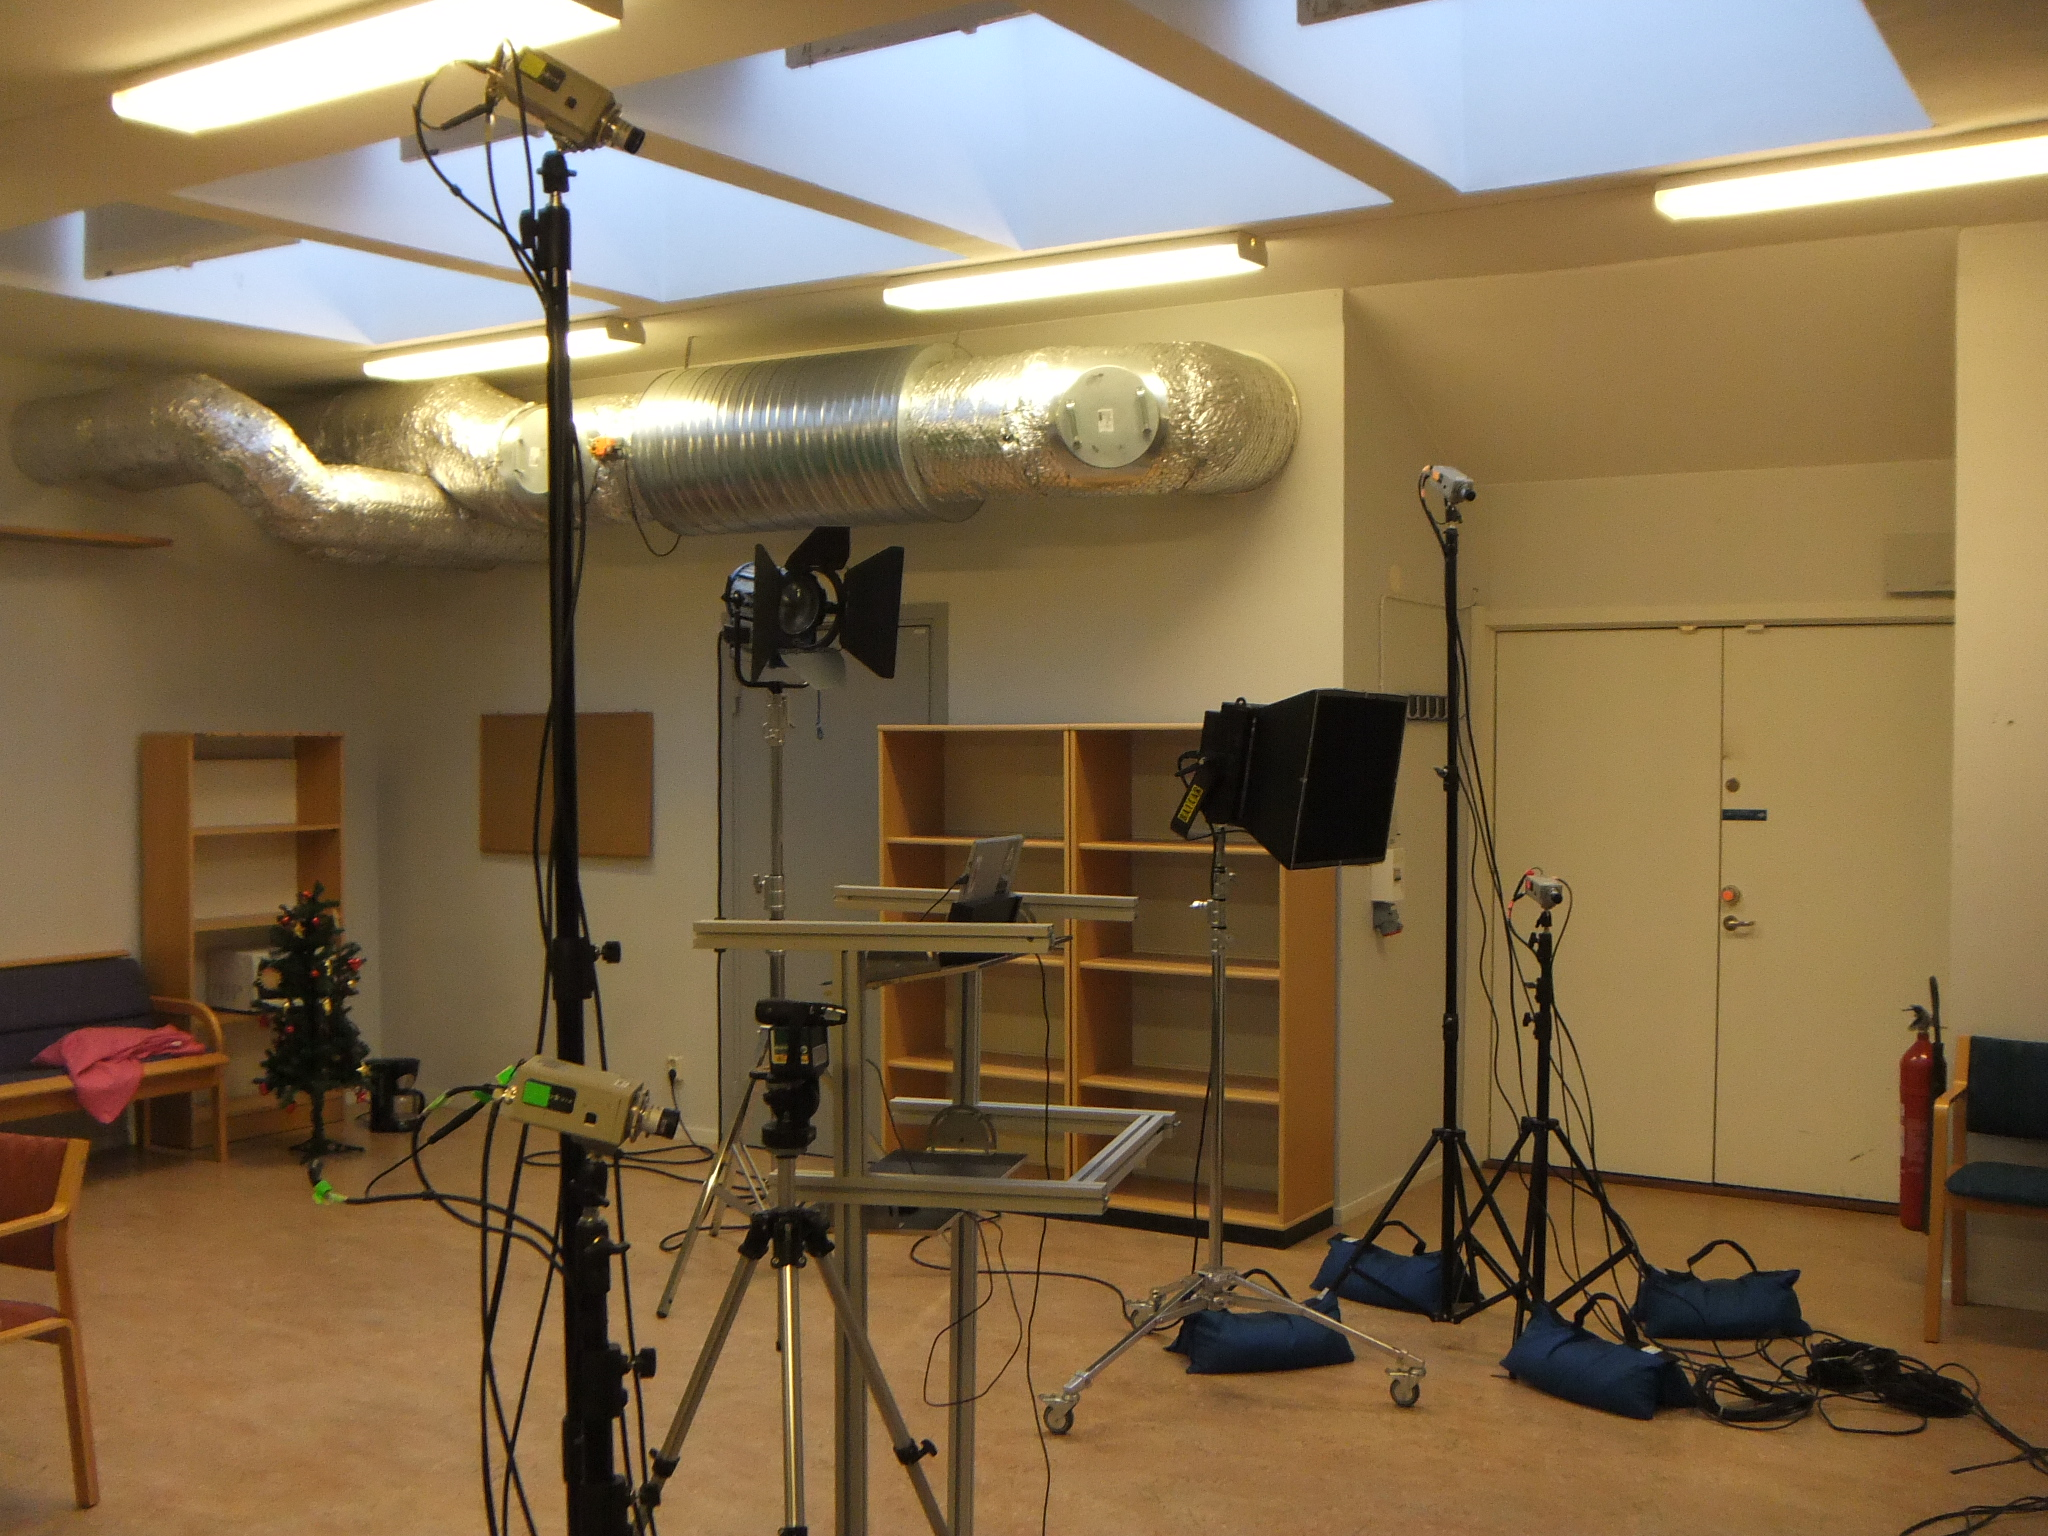
\includegraphics[width=0.6\textwidth]{figures/research/lab.jpg}
\caption{\label{fig:arlab} Eexperimental setup.} 
\end{figure}


\subsection{Forestry related applications}

	
	%--------------------------------------------------------------
	
	\item
	\textbf{Diffraction Artifact Reduction in \textmu CT Imaging}\\
	Erik Wernersson, Cris Luengo, Anders Brun, Gunilla Borgefors \\
	\ppartners{Jan Van den Bulcke, Dept.~of Forest and Water Management, Ghent University, Belgium; Matthieu Boone, Dept.~of Physics and Astronomy, Ghent University, Belgium}
	\ffunding{S-faculty, SLU}
	\pperiod{1009--1412}
	\aabstract{When imaging wood based materials, diffraction causes artefacts especially around sharp
		edges. While sometimes useful, and the only measurable properties of the imaged objects, they
		might as well be a nuisance which hinders proper analysis of the absorption coefficient. In this
		project, different ways to reduce such artefacts are investigated, especially in already reconstructed
		images. Compare to previous approaches, this is much faster and does not require that the original
		projection images are stored.
		
		This year we presented a paper at SSBA that showed how to tune the parameters of the method that
		we published in the Journal of the Optical Society of America A (2013). Erik Wernersson defended his PhD thesis closely related to this project in December 2014.}
	
	
	%--------------------------------------------------------------
	
	\item 
	\label{proj:paper}
	\textbf{Image Analysis of the Internal Structure of Paper and Wood Fibre Based Composite Materials in 3D~images}\\% \textcolor{red}{To Be Removed If No Updates}}\\
	Erik Wernersson, Anders Brun, Cris Luengo, Gunilla Borgefors\\
	\ppartners{Gary Chinga, Norwegian Pulp and Fibre Research Institute, Trondheim, Norway;
		Catherine \"{O}stlund, Innventia, Stockholm; Thomas Joffre, Dept.~of Engineering Sciences, Applied
		Mechanics, UU; Arttu Miettinen, Dept.~of Physics, University of Jyv\"{a}skyl\"{a} (UJ), Finland;  Joakim Lindblad, University of Novi Sad, Serbia; Svetlana Borodulina, Dept.~of Solid Mechanics and BiMaC Innovation Center, KTH
	}
	\ffunding{S-faculty, SLU; WoodWisdom-Net}
	\pperiod{0406--1412}
	%\newpage
	\aabstract{The internal structure of paper is important because many of its properties correspond
		directly to the properties of single fibres and their interaction in the fibre network. How single
		fibres in paper bond and how this affects paper quality is not fully understood, since most structure
		analysis of paper has been performed in cross-sectional, two-dimensional (2D) images whereas
		paper is a complex, three-dimensional (3D) structure.
		Another application for wood fibres that has recently gained interest is wood polymer
		composite materials. The properties of these materials do not only depend on the structure of the fibre
		network, but also on the interaction between the fibres and the polymer matrix surrounding the
		fibres.
		
		
		Advances in imaging technology have made it possible to acquire 3D images of paper and wood
		polymer composite materials. In this project, image analysis methods for characterising the 3D
		material structure in such images are developed. The detailed knowledge of the material structure
		attainable with these methods is useful for improving material properties and for developing new
		materials.
		
		The project objective is to achieve a complete segmentation of individual fibres and pores in
		volume images of the material. Given such a segmentation, any desired measurement of the internal
		structure is available. A sample segmentation result is shown in Figure \ref{fig:woodseg}. Measurements on individual fibres and the structural arrangement of fibres
		can then be related to macroscopic material properties.
		
		In this project, different volume images of paper and composite materials are available: one volume
		created from a series of 2D scanning electron microscopy (SEM) images at StoraEnso, Falun; and
		X-ray microtomography volume images of paper and composite samples imaged at the European
		Synchrotron Radiation Facility (ESRF) in Grenoble, France, at the Paul Scherrer Institut (PSI) in
		Villigen, Switzerland and also from tabletop scanners at University of Jyv\"{a}skyl\"{a}, Finland,
		at Applied Mechanics, Uppsala University, and at Innventia, Stockholm.
		
		This year we published papers in the Nordic Pulp \& Paper Research Journal,
		Cellulose, and the Mechanics of Materials. Erik Wernersson defended his PhD thesis closely related to this project in December 2014.}
	
	\begin{figure*}[!h]
		\centering
		
		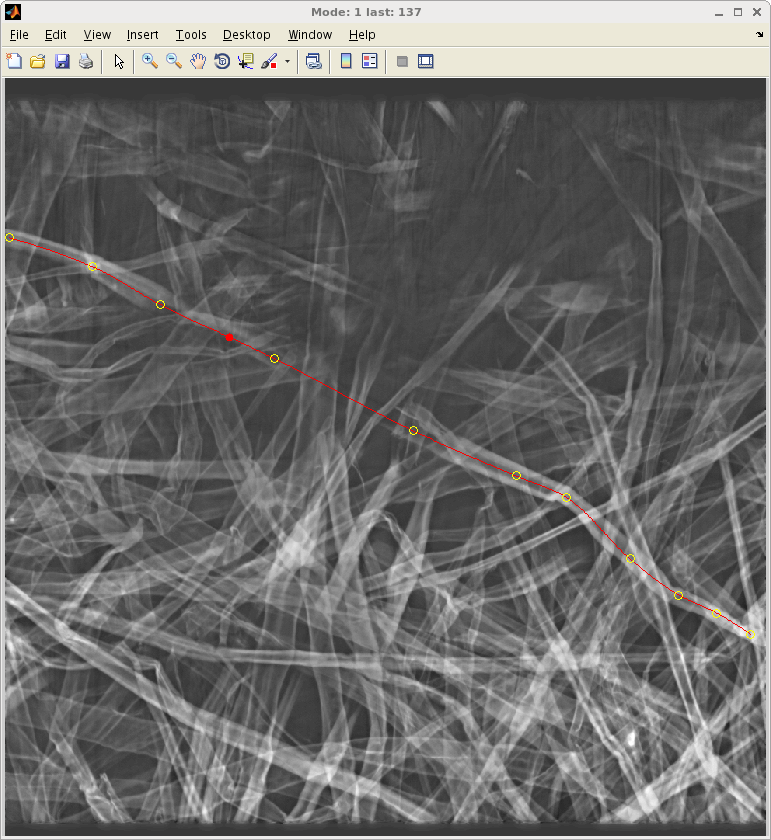
\includegraphics[width=0.48\linewidth]{figures/research/eric.png}
		\caption{Through an interactive tool, users can quickly select and trace fibres within a 3D image of a paper sheet. Here, a 2D projection parallel to the sheet is shown. [Taken from our paper in Nordic Pulp and Paper Research Journal 29(3) 2014, and also used as cover image for that issue.]}
		\label{fig:woodseg}
	\end{figure*}
	%----------------------------------------------------------------------------------------------------------------------------------------------
	
	
	
	
	
	%----------------------------------------------------------------------------------------------------------------------------------------------
	
	\item
	\textbf{Ring Width and Density Profiling with Helical CT}\\
	Erik Wernersson, Cris Luengo, Anders Brun, Gunilla Borgefors \\
	\ppartners{Jan Van den Bulcke, Dept.~of Forest and Water Management, Ghent University, Belgium}
	\ffunding{S-faculty, SLU}
	\pperiod{1201--1412}
	\aabstract{Dendrochronology relies on accurate measurements of annual ring widths. The most
		common method is to use a flatbed scanner to acquire high resolution images of polished wood
		surfaces. In this project we investigate potential gains using a helical X-ray device which produces
		volume images. Direct advantages include non destructive and simplified sample preparation procedures
		as well as compensation for the orientation of the inner structure which can not be seen
		with ordinary flatbed scans. It is also possible to find density profiles using the same images.
		
		One article was published in Dendrochronologia. Erik Wernersson defended his PhD thesis closely related to this project in December 2014.}
	
	%-------
%--------------------------------------------------------------------------------------

\newpage
	\item
	\textbf{Light Scattering in Paper}\\
	Erik Wernersson, Cris Luengo \\
	\ppartners{Tomas Linder and Torbj\"{o}rn L\"{o}fqvist, Lule\r{a} University of Technology, Lule\r{a}}
	\ffunding{S-faculty, SLU}
	\pperiod{1212--1412}
	\aabstract{Fibre orientation is an important structural property in paper and other fibrous materials.
		In this study we explore the relation between light scattering and in-plane fibre orientation
		in paper sheets. Light diffusion from a focused light source is simulated using a
		Monte Carlo technique where parameters describing the paper micro-structure were determined
		from 3D x-ray computed tomography images. Measurements and simulations on both spatially
		resolved reflectance and transmittance light scattering patterns show an elliptical shape
		where the main axis is aligned towards the fibre orientation.
		
		Good qualitative agreement was found at low intensities and the results indicate that
		fibre orientation in thin fibre-based materials can be determined using spatially resolved
		reflectance or transmittance. Published in Optics Express. Erik Wernersson defended his PhD thesis closely related to this project in December 2014.}
	%---------------------------------------------------------------------------------------------

\item
	\textbf{Large-scale quantification of gene expression in Arabidopsis}\\
	Azadeh Fakhrzadeh, Cris Luengo \\
	\ppartners{Urs Fischer, Hardy Hall, Ume\r{a} Plant Science Centre, SLU}
	\ffunding{S-faculty, SLU}
	\pperiod{1402--}
	\aabstract{Arabidopsis is the most important plant model organism. For animal model organisms such as Drosophila melanogaster (fruitfly), C.\ elegans 
(roundworm) and Danio rerio (zebrafish), efforts have been made to map gene 
expression on a per-cell or sub-cell resolution. In this project, we develop tools to create the first such map for a plant species. We prepare thin sections of the root, hypocotyl and stem of the plant at various stages between sprouting and maturity. These sections are fluorescently stained such that the cell 
walls can be visualized in the confocal microscope. Each section also receives a FISH (fluorescent in situ hybridization) stain for a particular protein. 
Sections are then imaged at a magnification that allows most of the section to fit in the field of view. This yields several thousand cells in each image. Next, we use a fully automatic segmentation and quantification pipeline that allows measurement of relative amount and quality of the stained protein in each 
subcellular area (wall and lumen are separated, and each divided into four regions: inner, outer and two lateral). Cells are automatically classified into the various cell types, which allows statistics of expression over each of the cell types, for example. We currently have imaged several thousand sections, from both wildtype and mutant samples, stained for hundreds of different genes (Figure \ref {fig:arabidopsis}).}

	\begin{figure*}[!h]
		\centering
		
		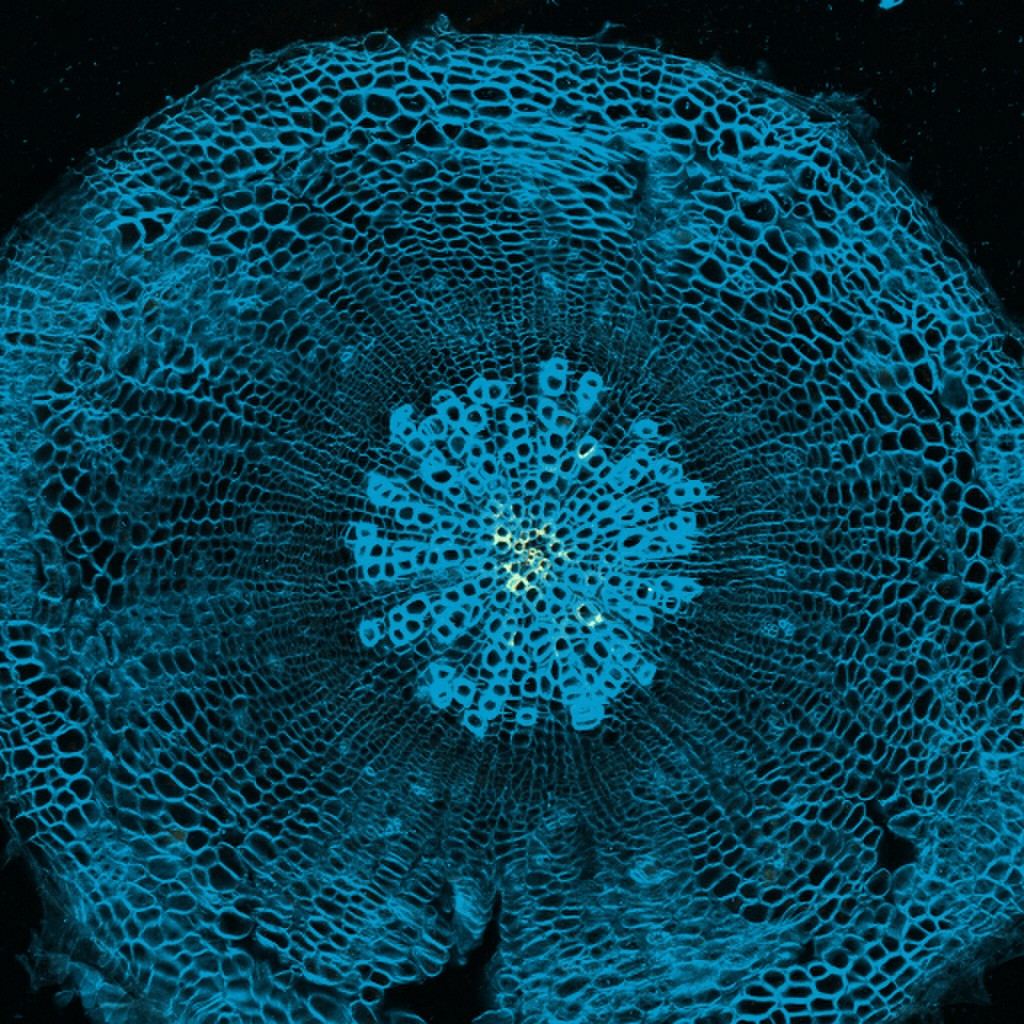
\includegraphics[width=0.48\linewidth]{figures/research/Arabidopsis.jpg}
		\caption{Cross section of the hypocotyl of a 21-day old Arabidopsis, 
stained for cell walls (blue) and a protein of interest (green).}
		\label{fig:arabidopsis}
	\end{figure*}

\subsection{Other applications}

\item \textbf{Writer Identification and Dating}\\
Fredrik Wahlberg, Anders Brun\\
\ppartners{Lasse M{\aa}rtensson, Dept.~of Business and Economics Studies, H\"{o}gskolan i G\"{a}vle}
\ffunding{UU; Swedish Research Council}
\pperiod{1401--}
\aabstract{The problem of identifying the writer of some handwritten text is of great interest in both forensic and historical research. Sadly the magical CSI machine for identifying a scribal hand does not exist. Using image analysis, statistical models of how a scribe used the quill pen on a parchment can be collected. These measurements are treated as a statistical distribution over writing practices. We using this information to identify single writers and perform style based dating of historical manuscripts.}

%-------------------------------------

\item \textbf{Optical Character Recognition of Handwritten Texts}\\
Anders Brun, Ewert Bengtsson, Fredrik Wahlberg, Tomas Wilkinson, Kalyan Ram\\
\ppartners{Lasse M{\aa}rtensson, Dept.~of Business and Economics Studies, H\"{o}gskolan i G\"{a}vle; Mats Dahll\"{o}f, Dept.~of Linguistics and Philology, UU; Alicia Forn\' es, Universitat Aut\` onoma de Barcelona, Italy}
\ffunding{Faculty of Languages and Humanities, UU; Swedish Research Council}
\pperiod{1008--}
\aabstract{Optical character recognition (OCR) is still, after nearly 100 years of research, an active area of research. Currently, one of the frontiers is the recognition of handwritten text (HTR), in particular from historical documents. This year, we had a two month visit by guest researcher Alicia Forn\' es from Universitat Aut\` onoma de Barcelona. We submitted several grant applications and continued a collaboration with the Swedish Museum of Natural History. Promising results during the year include a novel visualization technique, image based word clouds (Figure \ref{fig:OCR2}), large scale analysis of medieval letters, better techniques for document binarization and cluster analysis of letter shapes (Figure \ref{fig:OCR1}).}

\begin{figure}[!htbp]
	\centering
	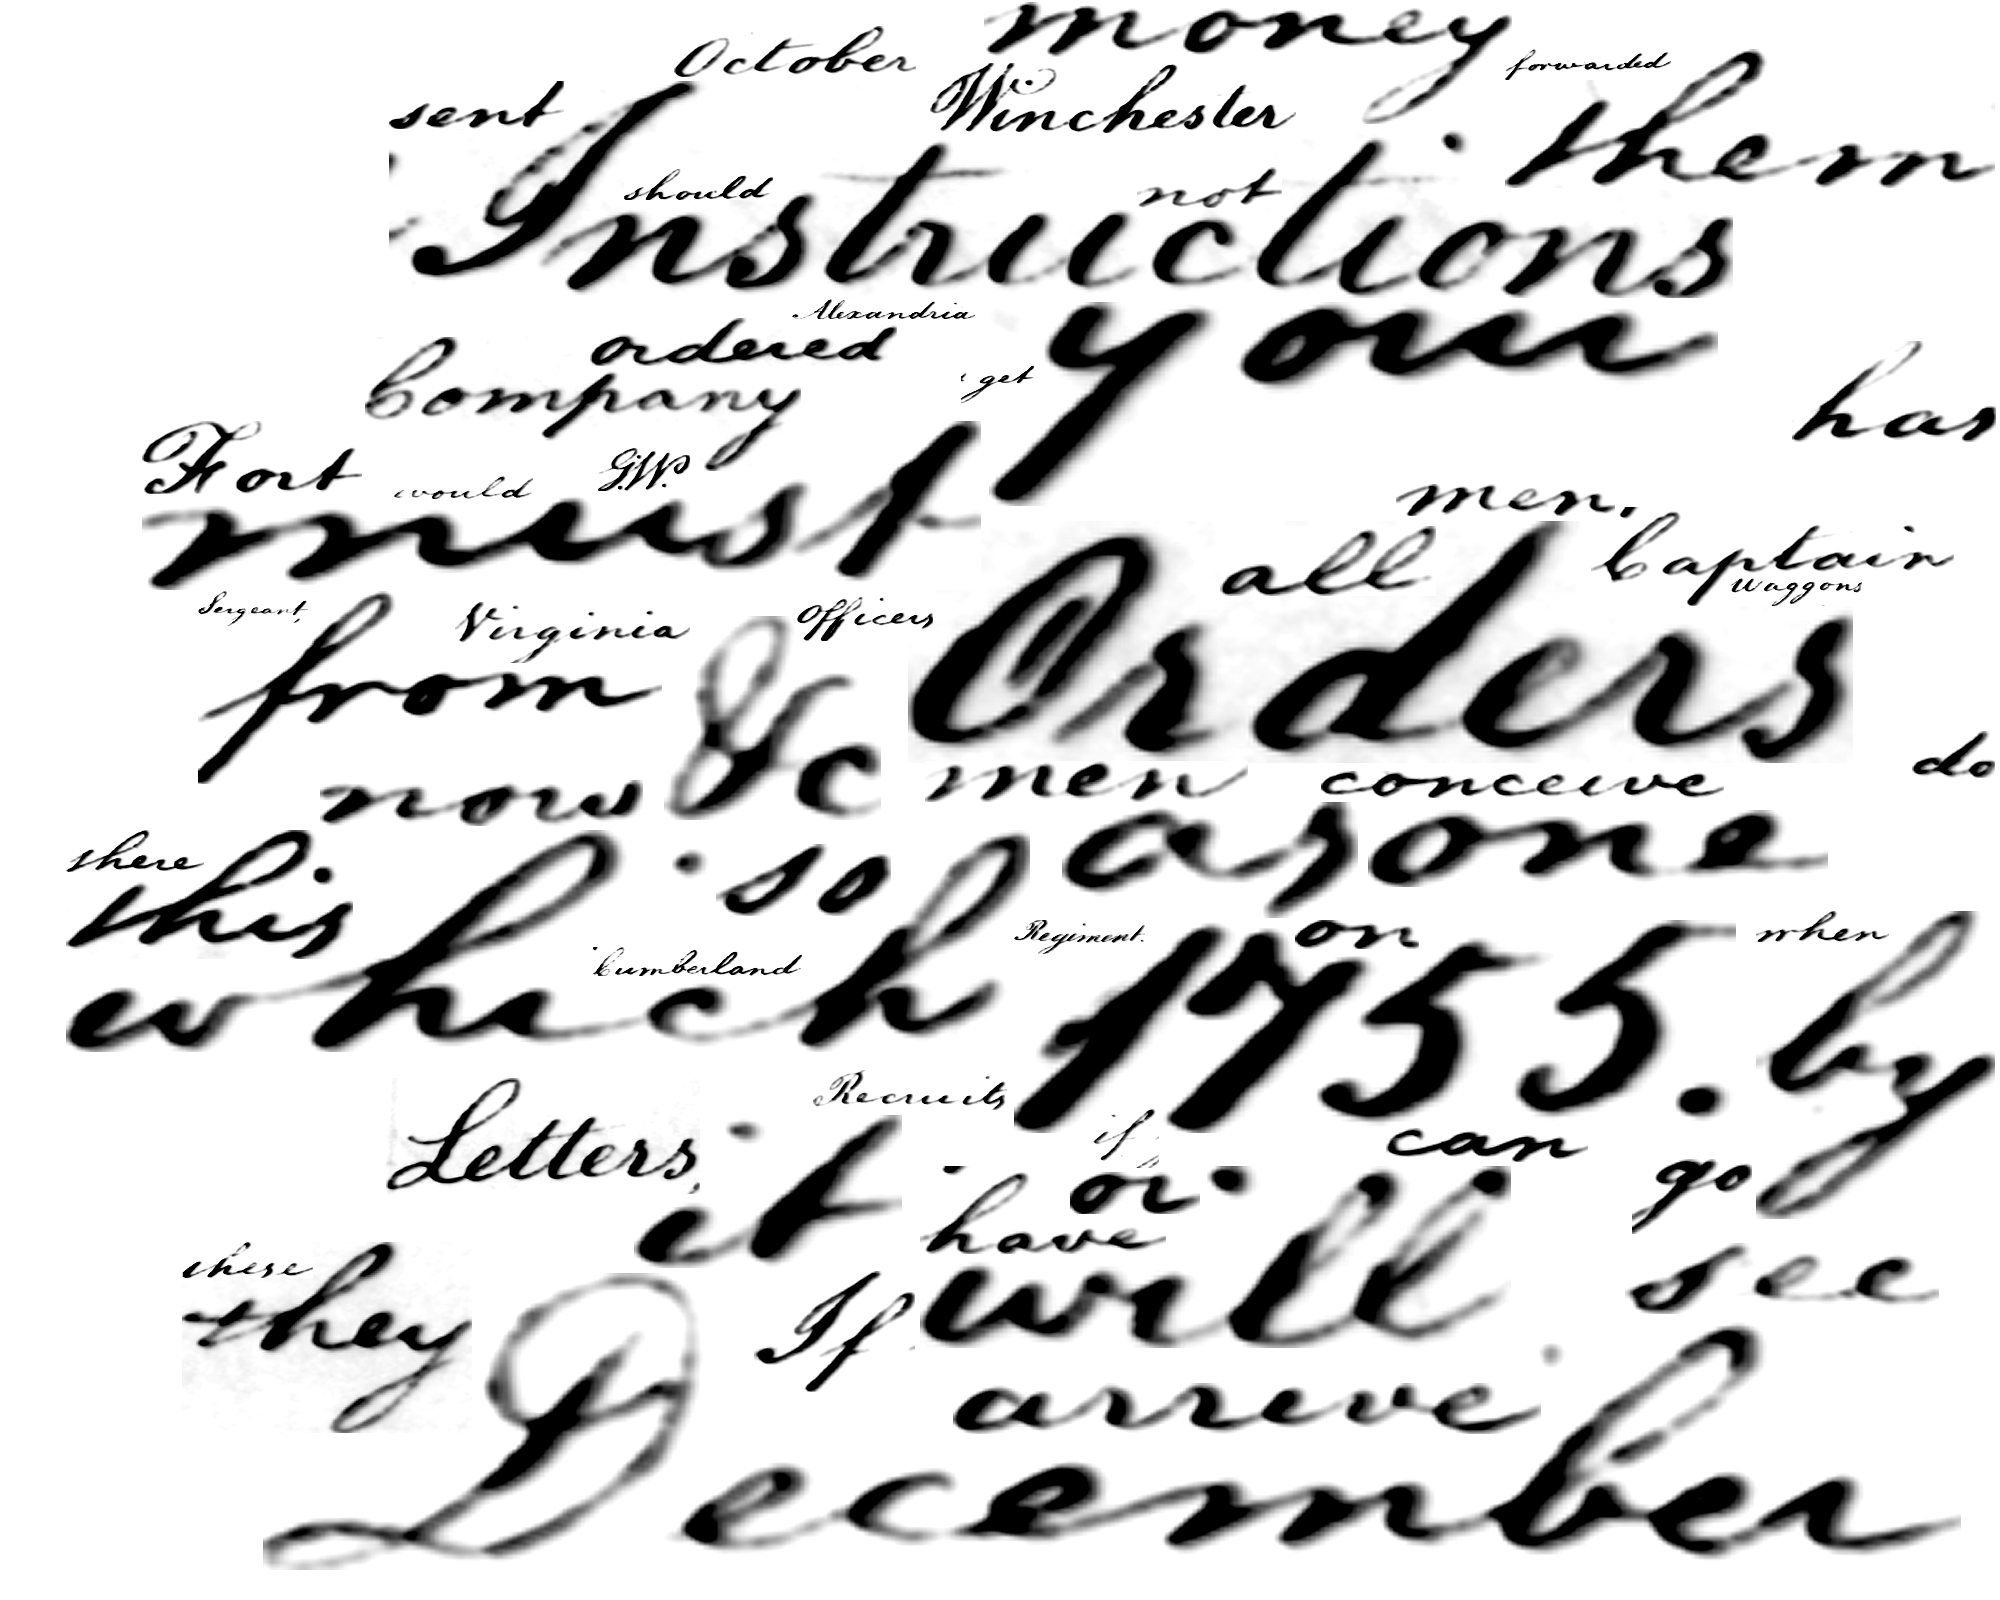
\includegraphics[width=0.6\textwidth]{figures/research/word_cloud_washington.png}
	\caption{\label{fig:OCR2} An image-based word cloud generated from a scanned collection of a 18th century letters written by George Washington. The cloud approximately contains the most frequently occuring images of words in the collection.} 
\end{figure}

\begin{figure}[!htbp]
	\centering
	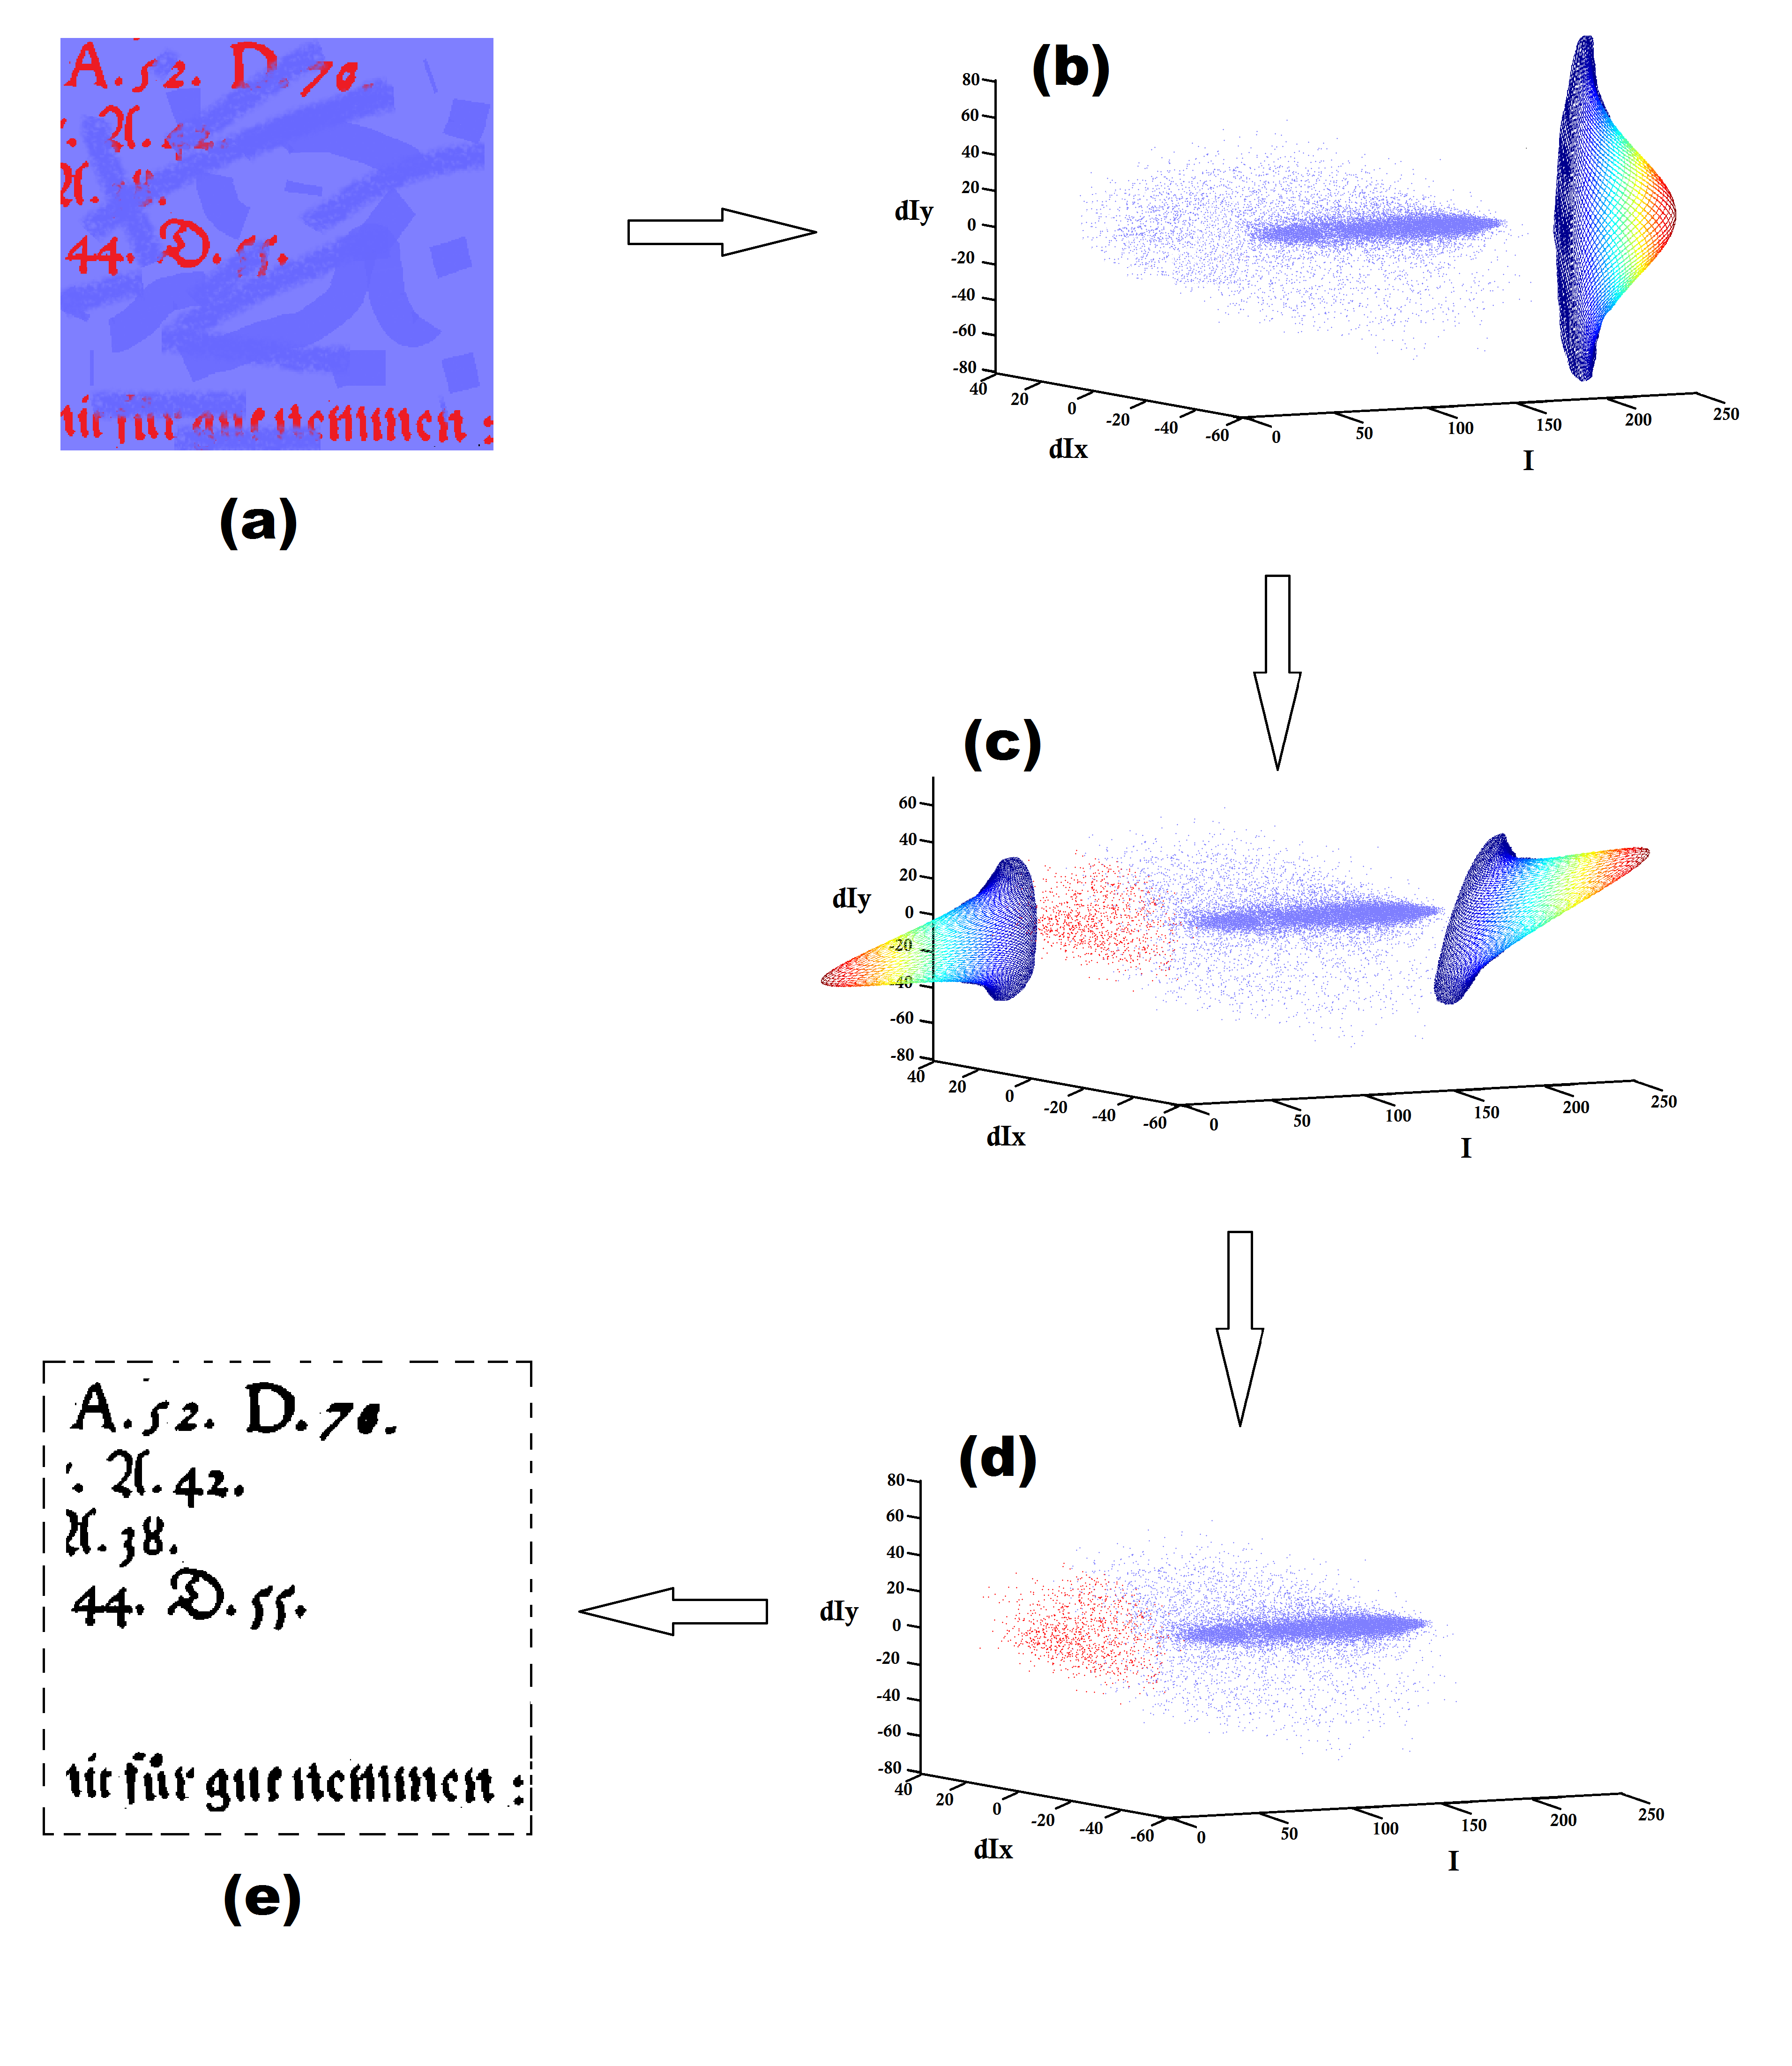
\includegraphics[width=0.6\textwidth]{figures/research/BgFgClus.png}
	\caption{\label{fig:OCR1} Hierarchical Mean Shift clustering based binarization procedure is outlined here with input as shown in (a) and output as indicated in (e) through separation of foreground and background clusters in a three dimentional space of intensity, $x$-derivative, $y$-derivative at each pixel as shown in (b)-(d).} 
\end{figure}

\item
\label{proj:geomemories}
\textbf{GeoMemories}\\
Anders Hast\\
\ppartners{Andrea Marchetti, Salvatore Minutoli, Alessandro Prosperi, Alessandro Lugari, Maurizio Tesconi, Beatrice Rapisarda, Matteo Abrate, Clara Bacciu, Davide Gazz\'e, Sergio Bianchi, Istituto di Informatica e Telematica (IIT), Pisa, Italy}
\aabstract{The GeoMemories project is aimed at making publicly available, through web access, heritage preserved in the archives of Aerofototeca Nazionale in Rome, which contains photographs covering the Italian territory from the end of 1800 till modern days. The web application is based on google earth but oriented towards the management of the temporal variable, so that geospatial changes can be monitored over time. The historical aerial photos need to be digitized, illumination corrected, orthorectified, georeferenced and finally stitched together. Anders Hast spent one year (2011) at IIT, CNR in Pisa Italy as an ERCIM fellow working with image processing and computer vision aspects in the project. Since returning to UU he is a research associate at IIT, CNR and continues working with the project and focus has been on how to improve the algorithms needed and several papers have been published. Recently the challenges and advantages of stereo visualisation of the historical archive has been investigated.}


\item \textbf{Image Analysis for Landscape Analysis}\\
Anders Brun\\
\ppartners{Bo Malmberg, Michael Nielsen, Dept.~of Human Geography, Stockholm University; Anders W\"{a}stfelt, Dept.~of Economics, SLU}
\ffunding{UU/SU}
\pperiod{0901--}
\aabstract{This project is a collaboration with researchers at SU and SLU. It aims to derive information about the landscape (rural and city) from satellite images. The project focuses on using texture analysis of images, rather than only pixelwise spectral analysis, to segment the image into different meaningful regions. One journal manuscript was published during 2014 and the collaboration with the GLEAN project at the Dept.~of Political Science at Stockholm University has continued.}

\item \textbf{Recognition and Image Analysis for Natural History Collections}\\
Anders Brun, Tomas Wilkinson\\
\ppartners{Stefan Daume, Swedish Museum of Natural History; Alicia Forn\' es, Universitat Aut\` onoma de Barcelona, Italy}
\ffunding{UU/SU}
\pperiod{1401--}
\aabstract{In this project we investigate ways to automatically interpret text labels, which are often handwritten, in large natural history collections. Examples of such collections include for instance herbarium sheets and collections of insects. It is estimated that we have around 33 million collected specimen in Sweden alone. Some of these have been digitized, in particular herbarium sheets, but the process is very labor intense. Addring automatic recognition of text, would speed up this process considerably and make the digitized data more useful for further data mining. During 2015, we were co-applicants for one large infrastructure grant proposal and Anders Brun gave an invited speech at the Swedish Natural History Museum Digitization Symposium.}


\item 
\label{proj:honey_bees}
\textbf{Tracking Honey Bees and their Interactions}\\
Cris Luengo\\
\ppartners{Olle Terenius, Ingemar Fries, Joachim Rodrigues de Miranda, Eva Forsgren, Barbara Locke, Dept.~of Ecology, SLU; Fredrik Liljeros, Dept.~of Sociology, Stockholm University}
\ffunding{{\AA}ke Wiberg Foundation; S-faculty, SLU}
\period{1003--}\\
\aabstract{In this project, we are creating a system in which we can observe a portion of a bee hive (containing about one thousand individuals, each tagged with a unique identifier on its back) over days or weeks. Bees will be free to enter and exit the hive, and the environment will be set up to be as natural as possible for the bees. The purpose is to observe the natural behaviour of the bees, and record the type and duration of interaction between individuals. During 2014, we applied for funding to continue this work.}

\subsection{General theory and tools}

\item
\label{proj:stochwatershed}
\textbf{The Stochastic Watershed}\\
Bettina Selig, Cris Luengo, Ida-Maria Sintorn, Filip Malmberg, Robin Strand\\
\ffunding{S-faculty, SLU}
\pperiod{1102--}
\aabstract{The stochastic watershed is a method recently presented that builds on the classical seeded watershed algorithm. It creates a probability density function for edges in the image by repeated applications of the seeded watershed with random seeds. Previously, we developed a perturbation-based approach to improve the properties of the algorithm: by adding noise to the input image at every application of the seeded watershed, we were able to avoid larger regions being split.

During 2014, we published an efficient, deterministic algorithm that computes the result that one would obtain after an infinite number of repetitions of the seeded watershed (Pattern Recognition Letters), as well as an efficient algorithm to convert this tree-based result back to all edges in the image's graph.

We also submitted a paper that describes a method to combine the perturbation-based approach with the deterministic algorithm. This combined method is much faster than the original perturbation-based method, and improves on its results slightly.}

\item 
\textbf{Adaptive Mathematical Morphology}\\
Vladimir \' Curi\' c, Cris Luengo, Gunilla Borgefors\\
\ppartner{Anders Landstr\"{o}m, Matthew Thurley, Lule\r{a} University of Technology, Lule\r{a}; S\'{e}bastien Lef\`{e}vre, University of South Brittany, Vannes, France; Jes\'{u}s Angulo, Santiago Velasco-Forero, Centre for Mathematical Morphology, MINES ParisTech, Fontainebleau, France}
\ffunding{Graduate School in Mathematics and Computing (FMB)}
\pperiod{1101--}
\aabstract{The construction of adaptive structuring elements that adjust their shape and size to the local structures in the image has recently been a popular topic in mathematical morphology. Despite that several methods for the construction of spatially adaptive structuring elements have been proposed, it is still an open problem, both from a theoretical and implementation point of view. We have proposed the salience adaptive structuring elements, which modify their shape and size according to the saliency of nearby edges in the image, as well as structuring element with a predefined shape that only changes size based on the saliency of nearby edges.

This year, we published an overview paper on adaptive mathematical morphology, in which we compared a few of the most important methods for constructing adaptive structuring elements, as well as theoretical advances on how to properly define morphological operators. Currently, we are working towards defining more complex morphological operators using adaptive structuring elements, such as an adaptive hit-or-miss transform. Vladimir \' Curi\' c defended his PhD thesis closely linked to this project in May 2014.}


\item 
\label{proj:DT}
\textbf{Digital Distance Functions and Distance Transforms} \\
Robin Strand, Gunilla Borgefors \\
\ppartner{Benedek Nagy, Dept.~of Computer Science, Faculty of Informatics, University of Debrecen, Hungary; Nicols Normand, IRCCyN, University of Nantes, France}
\ffunding{TN-faculty, UU; S-faculty, SLU}
\pperiod{9309--}
\aabstract{The distance between any two grid points in a grid is defined by a distance function. In this project, weighted distances have been considered for many years. A generalization of the weighted distances is obtained by using both weights and a \textit{neighborhood sequence} to define the distance function. The neighborhood sequence allows the size of the neighborhood to vary along the paths. 

In 2014, the work was focused on weight sequence distance functions, where weighted neighborhood sequences of infinte length are allowed.}

% EEE

\item 
\label{project:minimum_barrier_distance}
\textbf{The Minimum Barrier Distance }\\
Robin Strand, Filip Malmberg, Elisabeth Linn\'{e}r\\
\ppartners{ Punam K. Saha, Dept. of Electrical and Computer Engineering and the Dept. of Radiology, University of Iowa, IA, USA; Krzysztof C. Ciesielski, Dept. of Mathematics, West Virginia University, Morgantown, WV, USA; Dept. of Radiology, MIPG, University of Pennsylvania, PA, USA }
\ffunding{TN-faculty, UU}
\period 1103--\\
\aabstract{In this project, we introduce a distance function on a fuzzy subset that gives the minimum barrier that has to be passed to go from one point to another. Theoretical properties as well as efficient computational solutions for minimum barrier distance have been developed. An initial application of minimum barrier distance in image segmentation is presented. The experiments show that the minimum barrier distance is robust to noise and blur, and also seed point position, since it captures the total change in membership values across an interface instead of gradient as a measure of slope that is sensitive to noise and blur.

During 2014, a paper describing an efficient method for exact calculation of minimum barrier distance transforms was published in Computer Vision and Image Understanding. Another paper, published in the proceedings of the international conference on Discrete Geometry for Computer Imagery, investigated the stability of the minimum barrier distance with respect to seed point position.}

%FFF

\item
\label{proj:set_dist}
\textbf{Set Distances and their Application in Image Analysis}\\
Vladimir \' Curi\' c, Gunilla Borgefors, Nata\v sa Sladoje\\
\ppartner{Joakim Lindblad, Faculty of Technical Sciences, University of Novi Sad, Serbia}
\ffunding{Graduate School in Mathematics and Computing (FMB); TN-faculty, UU}
\pperiod{0908--1406}
\aabstract{We have, in 2014, concluded our study related to methods for
measuring distances between sets, summarizing the results in two journal
publications and in Vladimir's PhD thesis, successfully defended in May
2014. To measure how similar sets are can be useful for solving various
image analysis related problems, such as registration, image retrieval and
segmentation evaluation.

During the project, we have evaluated existing and developed new set distances
which are useful in image registration related problems. A new set
distance between crisp sets of points is presented and evaluated w.r.t. utiliziation
in rigid body registration of binary images, as well as for multi-modal
2D--3D registration of 2D histological sections of bone implant with corresponding
3D synchrotron radiation micro computed tomography (SR\textmu CT) bone implant volumes. This work is published in the Pattern Analysis and Applications journal.

We extended our study to fuzzy objects and proposed four novel point-to-set
distances defined for fuzzy or gray-level image data, two based on integration
of alpha cuts and two based on the fuzzy distance transform. We further
used these point-to-set distances to define distances between fuzzy sets.
Theoretical study and performance evaluation of the proposed distances con-
firm their excellent behaviour in template matching and object classification.
New distance measures enable inclusion of both spatial and intensity information,
which makes them applicable to texture matching problems as well. The results of this study are published in IEEE Transactions on Image Processing. Vladimir defended his PhD thesis closely linked to this project in 2014.}

% GGG

\item
\textbf{Direct Curvature Calculation of Surfaces in 3D Volumes }\\
Erik Wernersson, Cris Luengo, Anders Brun, Gunilla Borgefors \\
\ffunding{S-faculty, SLU}
\pperiod{1009--1412}
\aabstract{Curvature is known to be a useful local descriptor of 2D surfaces, embedded in 3D space. Not only for parametric surfaces but also estimated from objects in digital images with applications ranging from visualisation to segmentation. Within this project, we have studied curvature calculated from the structure tensor, in contrast to the most common methods which derive curvature directly from image differentials. Using the structure tensor, we were able to use non-standard derivative operators to determine curvature. We also used non-linear smoothing to create the structure tensor. These two modifications together allow for a more precise estimate of curvature in places where the curvature changes quickly, or where two surfaces of different curvature are close together. We also correctly determine the sign of the curvature, which allows us to distinguish concave and convex surfaces. This distinction is useful for example to differentiate the inner and outer surface of a wood fibre. Erik defended his PhD thesis closely linked to this project in December of 2014.}

% NEW NATASHA ENERGY MIN

\item
\textbf{Image Enhancement based on Energy Minimization}\\
Nata\v sa Sladoje\\
\ppartners{Joakim Lindblad, Buda Baji\' c, Faculty of Engineering, University of Novi Sad, Serbia}
\ffunding{Swedish Governmental Agency for Innovation Systems (VINNOVA); TN-faculty, UU}
\pperiod{1409--}
\aabstract{A common approach  to solve the very important but severely ill-posed problem of image deconvolution, is to formulate it in a form of an energy minimization problem. Typically, some regularization is applied, utilizing available a priori knowledge. Total variation regularization is among most popular approaches, due to its generally good performance. 

Within this project we are exploring different ways to improve the results of energy minimization based image deconvolution. During 2014 we have studied utilization of different {\em potential functions} in restoration of images degraded by both noise and blur. We have tested performance of seven known potentials, convex as well as non-convex, utilizing empirically determined optimal parameter settings for each of them. We have performed optimization  by a  flexible and efficient SPG method. Our study confirm that some appropriately chosen potentials provide a straightforward way to increase quality of the restored images. 

We have presented the results of our study at the International Conference on Image Analysis and Recognition (ICIAR 2014), held in Algarve, Portugal. 
The proceedings of the conference is printed in the Lecture Notes in Computer Science series.}

% NEW project NATSHA cover models

\item
\textbf{Coverage Model and its Application to High Precision Medical Image Processing}\\
Nata\v sa Sladoje\\
\ppartners{Joakim Lindblad, Faculty of Technical Sciences, University of Novi Sad, Serbia;  Attila Tan\' acs and Zoltan Kato, Dept. of Image Processing and Computer Graphics, University of Szeged, Hungary}
\ffunding{TN-faculty, UU}
\pperiod{1409--}
\aabstract{The coverage model, that we have been developing for several years now,  provides a framework for representing continuous objects present in digital images as spatial fuzzy subsets. Assigned membership values indicate to what extent image elements are covered by the imaged objects.  During last years, we have shown, both theoretically, and in applications, that the model can be used to improve information extraction from digital images and to reduce problems originating from limited spatial resolution. 

During 2014, we have finalized our study on a unified framework to recover linear geometric correspondences between binary objects in $n$-dimensions. The solution of the registration problem is obtained by solving polynomial systems of equations that are based on geometric moments of the template and observation, with no need for additional correspondences. 

To further improve the performance of this fast and efficient registration method, we have proposed to use coverage information to compensate for possibly insufficient spatial resolution and to reach the desired precision of moments estimates. The work is published in the Pattern Recognition journal, where the advantages of this approach are clearly demonstrated, in particular in terms of increased percentage of registration results in the highest scoring group. An illustration of the  proposed methods is demonstrated on real X-ray images of hip replacement implants and 3D CT volumes of the pelvic area (Figure \ref{fig:realct}).} 

\begin{figure}[]
%
\begin{minipage}[b]{.42\linewidth}
  \centering
\centerline{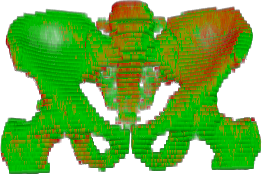
\includegraphics[width=\linewidth]{figures/research/cd03_0003_overlay_3d_gc}}
\vspace{1mm}
\end{minipage}
\hfill
\begin{minipage}[b]{0.42\linewidth}
  \centering
  \centerline{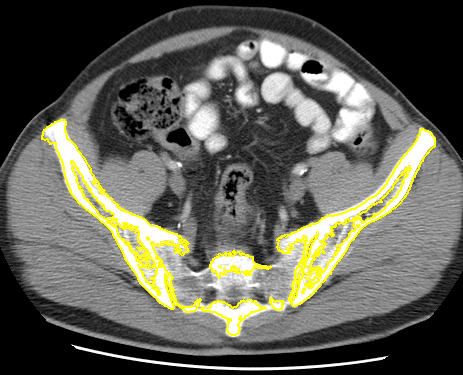
\includegraphics[width=\linewidth]{figures/research/d03_0003_Reg_Overlay_0015_cut}}
\vspace{1mm}
\end{minipage}\\
\begin{minipage}[b]{.42\linewidth}
  \centering
\centerline{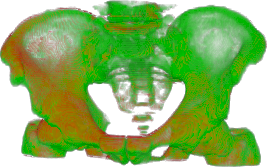
\includegraphics[width=\linewidth]{figures/research/sa_09_10_cut_3d_reg_overlay_gc}}
\vspace{1mm}
\end{minipage}
\hfill
\begin{minipage}[b]{0.42\linewidth}
  \centering
  \centerline{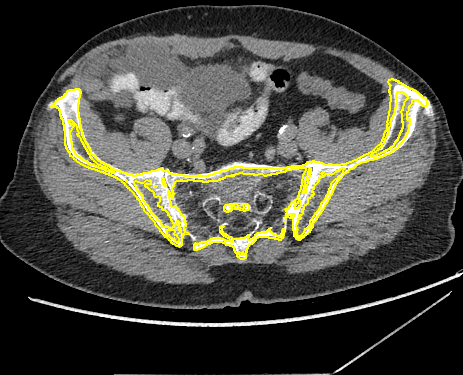
\includegraphics[width=\linewidth]{figures/research/SA_09_10_cut_Reg_Overlay_0056_cut}}
\vspace{1mm}
\end{minipage}
\caption{Registration of pelvic CT data: superimposed registered 3D bone
models (left column), and
bone contours of the registered template (yellow) overlaid on a CT slice of the observations (right column).
}
\label{fig:realct}
\end{figure}

\newpage

%
% Christer
% Project Digital Geometry

\item 
\textbf{Digital Hyperplanes}\\
Christer Kiselman\\
\ppartners{Adama Kon\' e, Universit\' e de Bamako}
\ffunding{International Science Programme; Universit\' e de Bamako; Kingdom of Sweden}
\pperiod{1011-}
\aabstract{Digital planes in all dimensions are studied, which means that digital straightness is in focus. The general goal is to generalize to any dimension the results of Kiselman's 2011 paper in Mathematika (Figure \ref {fig:crister2}).}

\begin{figure}[!htbp]
	\centering
	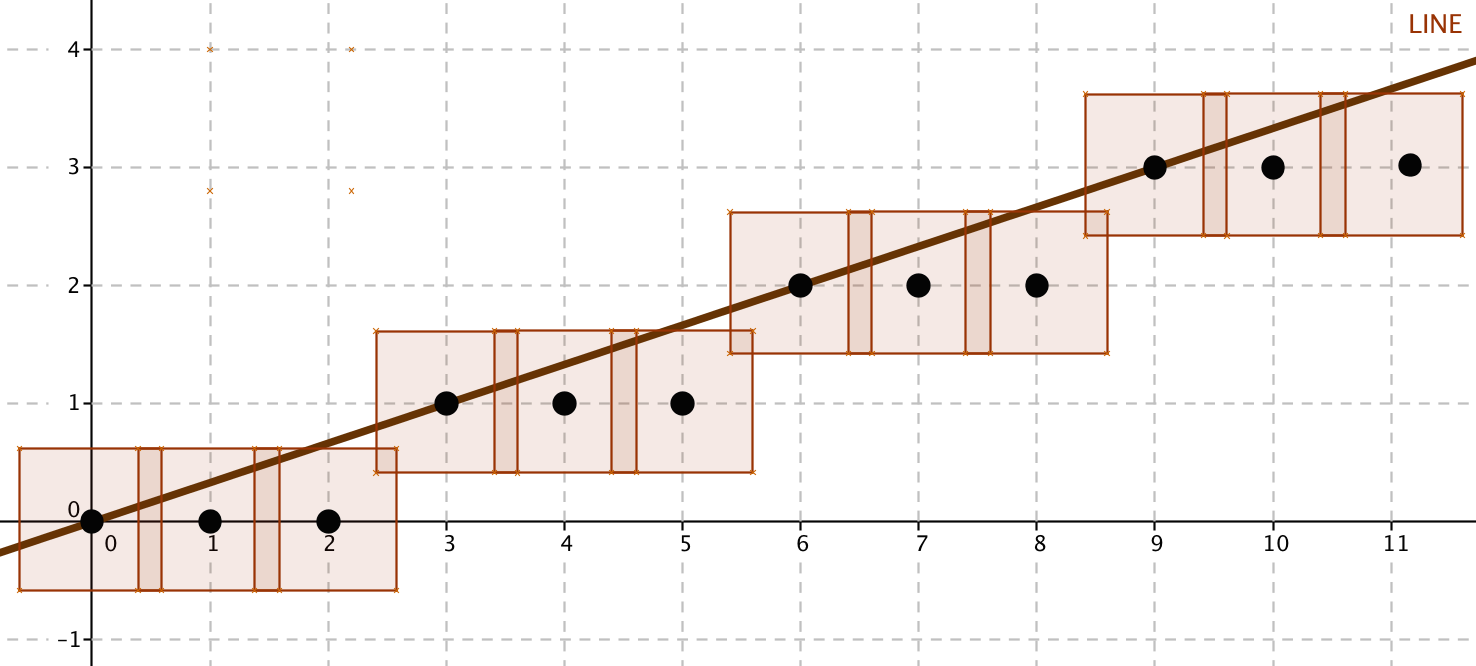
\includegraphics[width=0.8\textwidth]{figures/research/CoveringUFloor.png}
	\caption{\label{fig:crister2} The figure shows how a Euclidean straight line can, or cannot, be covered by dilations of one of its discretizations, in this case the discretization defined by the floor function.  The structuring element of the dilations is a rectangle.  The project concerns analogous results in higher dimensions.} 
\end{figure}



\item 
\textbf{Convexity of Marginal Functions in the Discrete Case}\\
Christer Kiselman\\
\ppartners{Shiva Samieinia, KTH}
\ffunding{Stockholm University; KTH; Kingdom of Sweden}
\pperiod{1011-}
\aabstract{We define, using difference operators, classes of functions defined on the set of points with integer coordinates which are preserved under the formation of marginal functions. The duality between classes of functions with certain convexity properties and families of second-order difference operators plays an important role and is explained using notions from mathematical morphology. A manuscript was submitted in 2014. Some problems remain to be solved (Figure \ref {fig:crister1}).}

\begin{figure}[!htbp]
	\centering
	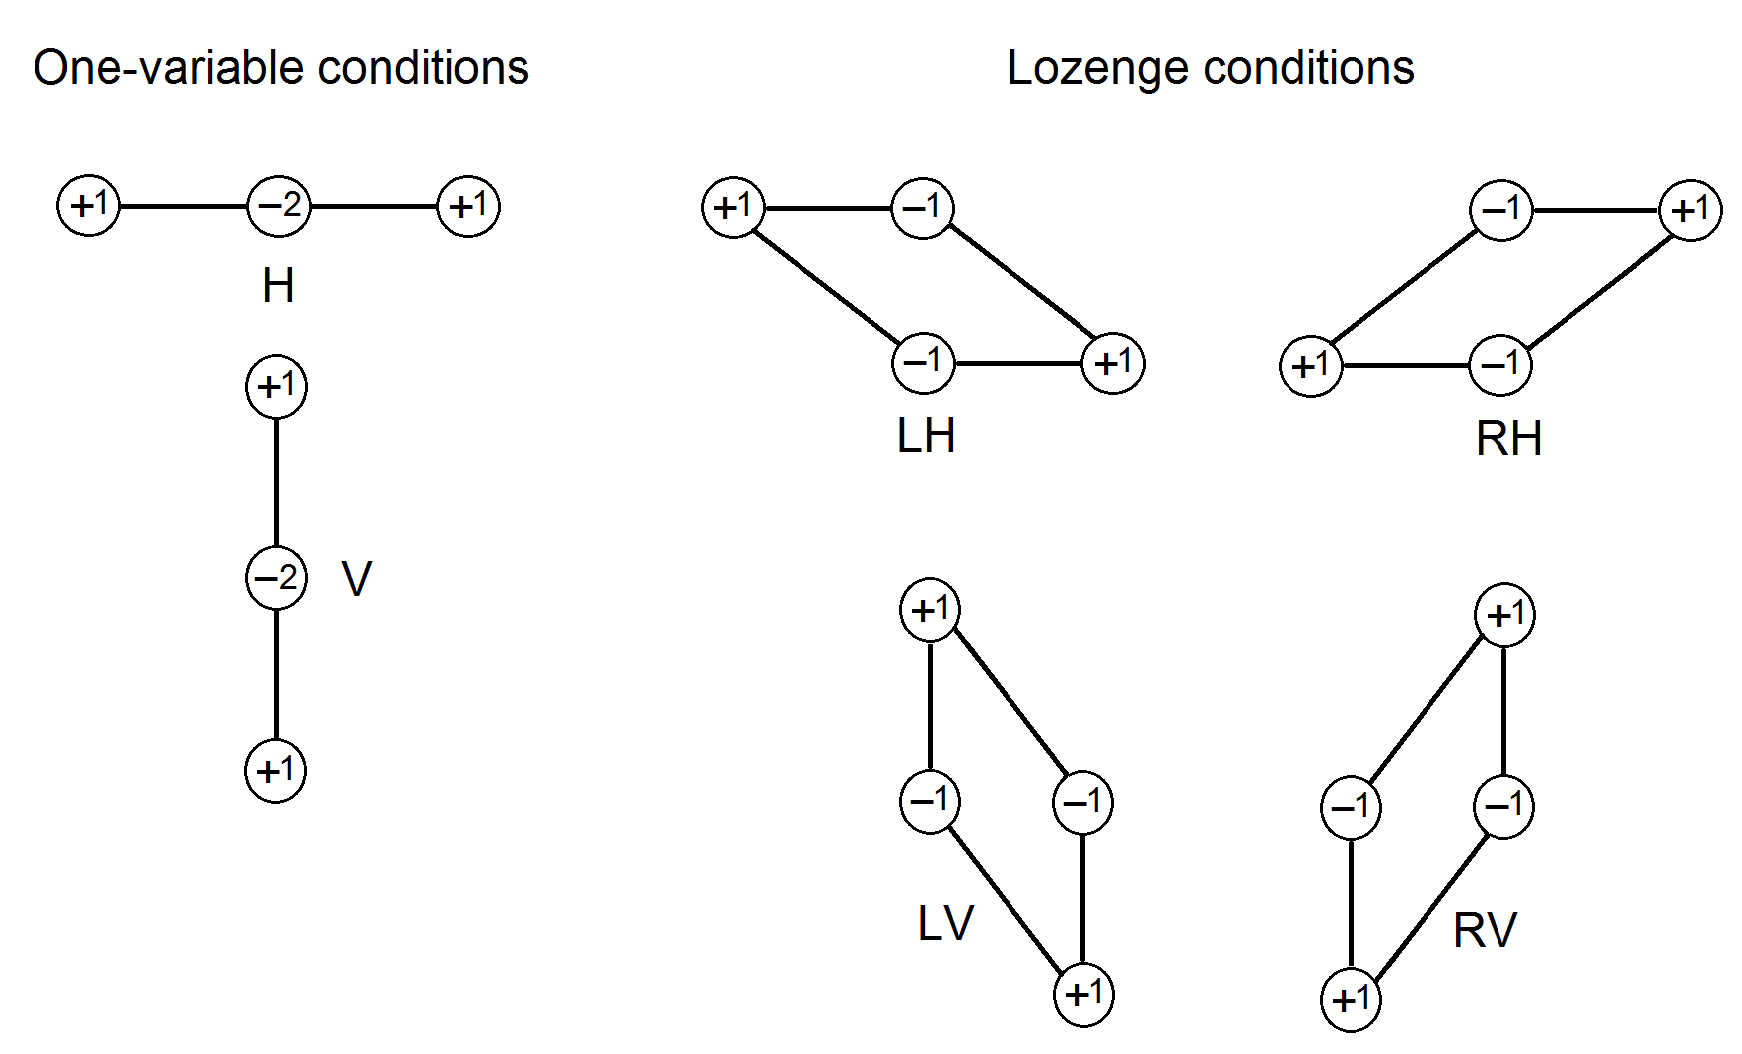
\includegraphics[width=0.8\textwidth]{figures/research/fig1new.png}
	\caption{\label{fig:crister1} The marginal function of a convex function of real variables is easily seen to be convex, but in the discrete case, nothing is obvious.  For a function of two integer variables, six conditions involving second-order difference operators are sufficient for its marginal function to be convex extensible.  The figure shows the weights in these difference operators.} 
\end{figure}

%
% Christer Project
% Euclid Straight Lines

\newpage

\item 
\textbf{Euclid's Straight Lines}\\
Christer Kiselman\\
\ffunding{Kingdom of Sweden}
\pperiod{0701-}
\aabstract{The project is both linguistic and mathematical. We raise two 
questions on Euclid's Elements: How to explain that Propositions 16 and 27 in his first book do not follow, strictly speaking, from his postulates (or are perhaps meaningless)? and: What are the mathematical consequences of the meanings of the term eutheia, which we today often prefer to consider as different? 

The answer to the first question is that orientability is a tacit assumption.  The answer to the second is rather a discussion on efforts to avoid actual infinity, and having to (in some sense or another) construct equivalence classes of segments to achieve uniqueness. An article will appear in Normat.}

%
% Christer
% Discrete Convolution Equations
\newpage
\item 
\textbf{Discrete Convolution Equations}\\
Christer Kiselman\\
\ffunding{Kingdom of Sweden}
\pperiod{1201-}
\aabstract{We study solvability of convolution equations for functions with discrete support in $\mathbf{R}^n$, a special case being 
functions with support in the integer points.  The more general case is of interest for several grids in Euclidean space, like the 
body-centred and face-centered tesselations of three-space, as well 
as for the non-periodic grids that appear in the study of 
quasicrystals.  The theorem of existence of fundamental solutions by de Boor, H\"{o}llig \& Riemenschneider is generalized to general discrete supports, using only elementary methods.  We also study the asymptotic 
growth of sequences and arrays using the Fenchel transformation. Estimates using the Fourier transformation will be studied later.}


\item
\label{proj:dipimage}
\textbf{DIPimage and DIPlib}\\
Cris Luengo\\
\ppartners{Bernd Rieger, Lucas van Vliet, Quantitative Imaging Group, Delft University of Technology, The Netherlands; Michael van Ginkel, Unilever Research and Development, Colworth House, Bedford, UK}
\ffunding{S-faculty, SLU}
\pperiod{0807--1412}
\aabstract{DIPimage is a MATLAB toolbox for scientific image analysis, useful for both teaching and research (\url{http://www.diplib.org}). It has been in active development since 1999, when it was created at Delft University of Technology. In 2008, when Cris Luengo moved to Uppsala, CBA was added to the project as a main development site. DIPlib, created in 1995, is a C library containing many hundreds of image analysis routines. DIPlib is the core of the DIPimage toolbox, and both projects are developed in parallel. Because DIPlib provides efficient algorithms, MATLAB is useful for image analysis beyond the prototyping stage. Together, MATLAB and DIPimage form a powerful tool for working with scalar and vector images in any number of dimensions.
	
	Versions 2.6 and 2.7 were released in 2014. Version 2.6 added the option to do arithmetic operations without changing the data type of the image, useful when working with very large images. We also fixed a major bug that appeared due to some undocumented internal change in MATLAB, which caused the output images of certain functions to be copied unnecessarily. Version 2.7 added the  possibility to record macros (as MATLAB M-files), added a few new functions, and fixed many bugs. In particular, we had to make many changes for compatibility with MATLAB's new graphic system.} 

% UPPMAX

\item 
\textbf{UPPMAX Cluster Computing}\\
Petter Ranefall, Ida-Maria Sintorn, Carolina W\"{a}hlby\\
\ppartners{Hans Karlsson, Elias Rudberg, Ola Spjuth, UPPMAX}
\ffunding{SciLife Lab Uppsala; eSSENCE; Dept.~of IT, UU}
\pperiod{1110-}
\aabstract{Life science applications generate a huge amount of image data that has to be stored and analysed in an efficient way. This project
	is focused on providing easy access to high-performance computers and large-scale storage. In collaboration with Uppsala Multidisciplinary Center for Advanced Computational Science (UPPMAX) image analysis software are being installed and maintained on the cluster. Database solutions with easy web access to image data are also being developed and maintained. This project has also provided workshops and seminars to help life science researchers to get started and use the resources. Several new large-scale image analysis projects using the computer cluster were initiated in 2014.}


\clearpage

%----------------------------------------------------------------------------------------------------------------------------------------------
%----------------------------------------------------------------------------------------------------------------------------------------------
%----------------------------------------------------------------------------------------------------------------------------------------------

\end{enumerate}

\end{document}

